\section{Mengenlehre}

\glqq Aus dem Paradies, das Cantor uns geschaffen, soll uns niemand vertreiben können.\grqq{}\\
(David Hilbert, 1926) 

\subsection{Mengen und Klassen}

Reine Mengen sind Kollektion an Objekten, die ebenfalls wieder Mengen sind, als Alternative lassen sich Mengen ausgehend von Urelementen definieren.
\\
Wie führt die Mathematik Objekte ein?
\begin{itemize}
	\item Explizite Konstruktion aus schon vorhandenen Objekten, bspw. Konstruktion der rationalen, reellen und komplexen Zahlen, ausgehend von den ganzen und natürlichen.
	\item Axiomatisches formulieren von gewünschten Eigenschaften der Objekte und betrachte alle Objekte, die die Eigenschaften erfüllen, bspw. Gruppen, Vektorräume, ...
\end{itemize}

\begin{definition}[Mengen]
	Intuitiv sind Mengen \textit{Kollektionen von Objekten}, die selbst wieder Mengen sind. 
	
	$a\in b$: $a$ ist ein Element in der Menge $b$.
	
	$a \subseteq b$: Jedes Element von $a$ ist auch in $b$.
	\\
	Eine Konstruktive Definition von aller Menge könnte wie folgt aussehen:\\ $\{\emptyset\}, \{\emptyset,\{\emptyset\}\}, \{\{\emptyset\}\}$ \textit{usw.}
	Problem: Wie sieht dieses \textit{usw.} aus?
\end{definition}


Mengen lassen sich auch als Bäume darstellen. Dies lässt sich in Abbildung \ref{Mengenbaum} Beispielhaft für die Menge $\{\; \emptyset, \; \{\emptyset\}, \; \{\emptyset,\{\emptyset\}\}\;\}$ erkennen. 

\begin{figure}[h]
	\begin{center}
		\begin{tikzpicture}
			\node {$\bigcirc$}
			child {node {$\emptyset$}}
			child {node {$\bigcirc$}
				child {node {$\emptyset$}}}
			child {node {$\bigcirc$}
				child {node {$\emptyset$}}
				child {node {$\bigcirc$}
					child {node {$\emptyset$}}}};
		\end{tikzpicture}
	\end{center}
\caption{Darstellung der Menge $\{\; \emptyset, \; \{\emptyset\}, \; \{\emptyset,\{\emptyset\}\}\;\}$ als Baum}
\label{Mengenbaum}
\end{figure}

\begin{definition}[Hereditär endliche Mengen]
	Die \textit{hereditär endlichen Mengen} ($HF$) bilden eine Miniaturversion der Mengenlehre. Es gilt $HF_0\subset HF_1 \subset HF_2 \subset \dots$. Definiert sind diese Mengen induktiv als $HF_0\coloneqq \emptyset$ und $HF{n+1}\coloneqq \{x : x\subseteq HF_n\}$, so dass $HF_{n+1}$ die Potenzmenge von $HF_n$ ist.
	
	Eine Menge ist hereditär endlich, wenn sie Element einer Menge $HF_n$ für ein $n$ ist. Weiter wird $HF\coloneqq\{x : x \in HF_n \text{ für ein }n\in \mathbb{N}\}$ definiert.
	Dies wirft folgende Frage auf: Ist $HF$ eine Menge? 
\end{definition}

Die ersten $HF$ Mengen lauten $HF_0=\emptyset$, $HF_1=\{\emptyset\}$, $HF_2=\{\emptyset,\{\emptyset\}\}$, \\ $HF_3=\{\emptyset, \{\emptyset\}, \{\{\emptyset\}\}, \{\emptyset,\{\emptyset\}\}\}$. Es lässt sich erkennen, dass $HF_n\subset HF_{n+1}$ und $HF_n\in HF_{n+1}$ für ein beliebiges $n$. Auch ist es möglich zu folgern, dass $HF_n$ endlich viele Elemente besitzt und jede Menge $a\in HF_{n+1}$ die Gestalt $a=\{b_0,\dots,b_{k-1}\}$ mit $b_0,\dots,b_{k-1}\in HF_n$. Außerdem gilt, dass $HF$ nicht hereditär endlich ist.

\begin{definition}[Natürliche Zahlen]
	Eine \textit{natürliche Zahl} $n$ ist definiert als $[n]\coloneqq\{[0],\dots,[n-1]\}$, wobei $[0]=\emptyset$ gilt. Die Menge der natürlichen Zahlen $\mathbb{N}$ lässt sich nun als $\mathbb{N}\coloneqq\{[n] : n \text{ eine nat. Zahl}\} \notin HF$. Eine Folgerung ist $[n]\in HF_{n+1}\setminus HF_n$.
\end{definition}

\subsubsection{Axiomensysteme für die Mengenlehre}

Das Modell der Mengenlehre besteht aus einer Kollektion $\mathcal{S}$ von Objekten, die wir Mengen nennen und einer Beziehung $\in$ zwischen diesen Objekten, so dass alle Axiome des Axiomensystems erfüllt werden.

\begin{definition}[Extensionalitätsaxiom (Ext.)]
	Zwei Mengen sind gleich, genau dann, wenn sie die selben Elemente haben. In einer Formel aus der Prädikatenlogik mit Signatur $\{\in\}$ wäre dies $\forall x \forall y (x=y \leftrightarrow \forall z (z \in x \leftrightarrow z \in y))$.
	\label{ExtAxiom}
\end{definition}

Die \textit{Konsistenz} des Axiomensystems der Mengenlehre beschreibt, ob es ein Modell des Axiomensystems gibt oder ob dieses Widersprüchlich ist. Es ist nicht möglich, die Konsistenz unseres Axiomensystems zu beweisen.

Das Axiomensystem der Mengenlehre ist \textit{Vollständig}, wenn alle Modelle \glqq gleich \grqq{} sind, in dem Sinn, dass die gleichen Eigenschaften gelten. Es gibt kein vollständiges Axiomensystem für die Mengenlehre.
\\
\\
Nehmen wir an, dass $(\mathcal{S},\in)$ ein beliebiges, aber festes Modell der Mengenlehre ist. Die Axiome sollen regeln, welche Kollektionen von Elementen aus $\mathcal{S}$ selbst wieder Elemente von $\mathcal{S}$, also Mengen sind. Dabei werden Kollektionen \textit{Klassen} genannt und Klassen, die keine Mengen sind, werden als \textit{echte Klassen} bezeichnet.

\begin{definition}[Die naive Mengenlehre]
	Das Axiomensystem der naiven Mengenlehre besitzt zwei Axiome. Zum einen das Extensionalitätsaxiom (siehe Definition \ref{ExtAxiom}) und das Axiomenschema der vollen Komprehension. Dieses besagt, dass sich für jede Formel $\psi(x)$ die Menge $\{x : \psi(x)\}$ bilden lässt: $\exists z \forall z(x \in z \leftrightarrow \psi(x))$.
\end{definition}

\begin{satz}[Zermelo-Russel Paradoxon]
	Die naive Mengenlehre ist inkonsistent.
	
	Sei $\psi(x)\coloneqq x\notin x$. Nach dem Komprehensionsschema muss nun folgende Formel gelten: $\exists z \forall x(x\in z \leftrightarrow x\notin x)$, aus welcher die Menge $z=\{x : x\notin x\}$ folgt. Eine solche Menge kann aber nicht existieren, da sonst $z\in z \Leftrightarrow z \notin z$ gelten müsste. Es folgt, dass $\{x:x\notin x\}$ immer einer echte Klasse sein muss.
\end{satz}

\begin{definition}[Das Axiomensystem ZFC]
	Das Axiomensystem ZFC (\textbf{Z}ermelo-\textbf{F}raenkel-\textbf{C}hoice) ist das heutzutage benutzte Axiomensystem. Es besitzt die folgenden Axiome:
	\begin{itemize}
		\item Das Extensionalitätsaxiom
		\item Das Aussonderungsaxiom: $\forall z \exists y \forall x (x\in y \leftrightarrow(x\in z \land \psi(x)))$. Dieses ist eine schwächere Version des Komprehensionsschemas, bei dem eine Menge aus bereits bestehenden Menge ausgewählt wird.
		\item Das Erzeugungsaxiom (Kreationsaxiom): Für jede Menge $x$ ex. eine \textit{Stufe} $s\in S$ mit $x\in s$.
		\item Das Unendlichkeitsaxiom: Es gibt eine \textit{Limesstufe} und damit eine unendliche Menge.
		\item Das Ersetzungsaxiom: Für jede Funktion $F:\mathcal{S}\to \mathcal{S}$ mit der Eigenschaft, dass wenn $Def(F)$ eine Menge ist, ist auch $Bild(F)$ eine Menge.
		\item Das Auswahlaxiom: Auf jeder Menge ex. eine \textit{Auswahlfunktion}
	\end{itemize}
\end{definition}

\begin{definition}[Klassenoperatoren]
	Seien $A, B$ Klassen.
	
	$A \subseteq B$: Jede Menge aus $A$ ist auch in $B$.
	
	$\bigcap A\coloneqq\{x : x\in y \text{ für alle } y \in A\}$
	
	$A \cap B \coloneqq \{x : x\in A \text{ und } x \in B\}$
	
	$A \setminus B \coloneqq \{x : x \in A \text{ aber } x \notin B\}$
\end{definition}

Für eine Formel $\psi(x)$ kann $\{x : \psi(x)\}$ entweder eine Menge oder eine echte Klasse sein. Somit lässt sich das Aussonderungsaxiom umformulieren: Für jede Menge $a$ und jede Klasse $A$ ist $a \cap A$ eine Menge. Daraus folgt, dass auch $a \setminus A$ eine Menge sein muss, dass $\bigcap A$ eine Menge ist, falls $A$ mindestens eine Menge enthält und, dass $\bigcap \emptyset = S$ keine Menge ist.

\subsection{Stufen und Geschichten}

Eine mögliche Methode zur Definition der gesamten Klasse aller Mengen ist es, die induktive Konstruktion der $HF$ zu erweitern. So ist $\mathcal{S}$ dann die Vereinigung einer aufsteigenden Folge von Mengen $S_\alpha$, welche wir die Stufen von $\mathcal{S}$ nennen. Es gilt $S_0\coloneqq \emptyset$ und für die bereits definierte Stufe $S_\alpha$ setzen wir $S_{\alpha +1}\coloneqq\{x : x\in S_\alpha\}$.

Sobald eine unendliche Folge von solchen Stufen definiert wurde, lässt sich eine neue Stufe als Vereinigung aller bisherigen Stufen definieren.\\

$S_0=HF_0=\emptyset$, $S_1=HF_1$, $\dots$, $S_n=HF_n$

$S_\omega \coloneqq \bigcup\limits_n S_n = \bigcup\limits_n HF_n = HF$

$S_{\omega+1}\coloneqq\{x : s\in S_\omega\}$, $\dots$

$S_{\omega+\omega}\coloneqq\{x : x \in S_{\omega+n} \text{ für ein } n\}$ \textit{usw.}

\begin{definition}[Die Akkumulation]
	Sei $A$ eine Klasse. Die \textit{Akkumulation} von $A$ ist $acc(A)\coloneqq\{x : (\exists y \in A) x\in y\lor x \subset y\})$.
\end{definition}

Da für eine Klasse $A$ und ein Element $a\in A$ natürlich gilt, dass $a \subset a$, gilt auch $a\in acc(A)$ und somit $A\subseteq acc(A)$.

\begin{definition}[Geschichten]
	Eine \textit{Geschichte} ist eine Klasse $H$, so dass für alle $a\in H$ gilt $acc(a\cap H)=a$.
\end{definition}

Die Stufe mit Geschichte $H$ ist $S\coloneqq acc(H)$.

\begin{example}[Beispiele zu Geschichten und Stufen]
	Im Folgenden soll für einige Mengen ihre Akkumulation gezeigt werden und bewiesen, dass es sich bei diesen auch um Geschichten handelt.
	\begin{itemize}
		\item $acc(\emptyset)=\emptyset$. $\emptyset$ ist eine Geschichte und die Stufe mit Geschichte $\emptyset$ ist $\emptyset$.
		\item $\{\emptyset\} = [1] = HF_1 = \{HF_0\}$: $acc(\{\emptyset\}) = \{\emptyset\}$. 
		$\{\emptyset\}$ ist auch eine Geschichte, denn für das einzige Element $\emptyset$ gilt $acc(\emptyset \cap \{\emptyset\})=acc(\emptyset)=\emptyset$. 
		Die Stufe mit Geschichte $\{\emptyset\}$ ist $\{\emptyset\}$.
		\item $\{\emptyset, \{\emptyset\}\}=[2]=HF_2=\{HF_0, HF_1\}$: $acc(HF_2)=HF_2$.
		$HF_2$ ist eine Geschichte, denn $acc(\emptyset \cap \{\emptyset, \{\emptyset\}\})=acc(\emptyset)=\emptyset$ und $acc(\{\emptyset\}\cap \{\emptyset, \{\emptyset\}\})=acc(\{\emptyset\})=\{\emptyset\}$. Die Stufe mit Geschichte $\{\emptyset, \{\emptyset\}\}$ ist $\{\emptyset, \{\emptyset\}\}$.
	\end{itemize}
\label{GeschichtenBsp}
\end{example}

Dies wirft die Frage auf, ob es eine Verallgemeinerung gibt. Demnach soll nun überprüft werden, ob $[n]$ eine Geschichte ist, für jedes $n$ in den natürlichen Zahlen. Für $k<n$ müsste gelten, dass $acc([n]\cap[k])=acc([k])\stackrel{!}{=}[k]$. 
Aber $acc([k])$ enthält alle Teilmengen von $[k-1]$, für $k=4$ also alle Teilmengen von $\{[0],[1],[2]\}$, demnach auch $\{[0], [2]\}$. Es gilt aber, dass $\{[0],[2]\}\notin [k]$ und es folgt $acc([k])\neq[k]$. Für $n \geq 3$ ist $n$ also keine Geschichte.

Ist $HF_n$ eine Geschichte? Nein, denn $[n-1]\in HF_n$ und $acc([n-1]\cap HF_n)=acc([n-1])\neq[n-1]$.

Aber $G_n\coloneqq\{HF_0,\dots,HF_{n-1}\}$ ist eine Geschichte mit Stufe $HF_n$. Für $n=0,1,2$ wurde dies schon in Beispiel \ref{GeschichtenBsp} gezeigt. Sei dies für $G_n$ bereits bewiesen, wir zeigen dies nun für $G_{n+1}=G_n\cup\{HF_n\}$.
$G_{n+1}$ ist eine Geschichte, wenn für alle $k \leq n$ gilt: $acc(HF_k\cap G_{n+1})=HF_k$.
$HF_k \cap G_{n+1} = \{HF_0,\dots,HF_{k-1}\}=G_k$ und per Induktionsvoraussetzung gilt $acc(G_k)=HF_k$.

Also ist $G_{n+1}$ eine Geschichte. Die Stufe mit Geschichte $G_{n+1}$ ist $acc(G_{n+1})=acc(G_n\cup \{HF_n\})=acc(GF_n)\cup HF_n \cup \{x : x\subseteq HF_n\}=HF_n\cup HF_n \cup HF_{n+1} = HF_{n+1}$.

Dies gibt die Idee für die Rückrichtung: Für jede Stufe $S_\alpha$ soll gelten, dass sie die Geschichte $H(S_\alpha)=\{S_\beta : \beta < \alpha\}$ hat.

\begin{definition}[Minimales Element]
	Eine Menge $m\in A$ ist ein \textit{minimales Element} von $A$, wenn $m\cap A=\emptyset$, d.h. es gibt kein $a\in A$ mit $a\in m \in A$.
	
	Eine Menge $a$ ist fundiert, wenn jede Menge $b$ mit $a\in b$ ein minimales Element enthält. Der fundierte Teil von $A$ ist $fd(A)\coloneqq\{x\in A : x \text{ ist fundiert}\}$.
\end{definition}

\begin{example}[Beispiele für minimale Elemente und Fundiertheit]
	$\emptyset$ ist fundiert.
	
	$\{\emptyset\}$ ist ebenfalls fundiert. Sei $\{\emptyset\}\in b$. Wenn $\{\emptyset\}\cap b =\emptyset$ ist $\{\emptyset\}$ das minimale Element. Andernfalls ist $\{\emptyset\}\cap b=\{\emptyset\}$ und $\emptyset$ ist das minimale Element von $b$.
\end{example}

\begin{satz}
	Wenn $H$ eine Geschichte ist, dann enthält jede nicht-leere Teilmenge von $H$ ein minimales Element
\end{satz}
\begin{proof}
	Es sei $a\in b \subset H$ und $c=\{fd(x) : x \in a\cap b\}=\{y:y=fd(x)\text{ für } x\in a \cap b\}$.
	Wenn $c=\emptyset$, dann ist $a\cap b = \emptyset$ und $a$ ist das minimale Element von $b$.
	Sei $c\neq \emptyset$. Wir wollen zeigen, dass $c\subseteq fd(a)$.
	
	\begin{lemma}
		Sei $H$ eine Geschichte, mit $a,b\in H$ und $a\in b$. Dann muss $fd(a)\in fd(b)$ gelten. Ansonsten wäre $fd(a)\in acc(b\cap H)=b$, da $fd(a)\subseteq a \in b \cap H$. Also gilt mit der Voraussetzung $fd(a)\in b \setminus fd(b)$. Demnach ex. eine Menge $x$ mit $fd(a)\in x$ ohne minimale Elemente. Speziell ist $fd(a)$ kein minimales Element von $x$, d. h. $fd(a)\cap x \neq \emptyset$. Sei $y\in fd(a)\cap x$. Da $y\in fd(a)$ ist $y$ fundiert. Da $y \in x$ hat $x$ ein minimales Element. Dies ist ein Widerspruch zu der Aussage, dass $fd(a)\in b \setminus fd(b)$, es muss also $fd(a)\in fd(b)$ gelten.
	\end{lemma}

	Sei $y\in c$. Dann ist $y = fd(x)$ für ein $x\in a\cap b$. Aus dem Lemma folgt, dass $y\in fd(a)$. Also $c\subseteq fd(a)$.
	
	Wenn $y\in c \subseteq fd(a)$, dann ist $y$ fundiert und $c$ hat ein minimales Element $z$. Nach der Definition von $c$ ist dann $z=fd(x)$ für ein $x\in a\cap b$.
	
	Behauptung: $x$ ist das minimale Element von $b$. Wenn nicht, dann existiert ein $u \in x \cap b$. Da $u \in x \in a\cap b\subseteq a\cap H$ und $a\in H$ ist auch $u$ in $acc(a\cap H)=a$. Also $u \in a\cap b$ und daher $fd(u)\in c = \{fd(x):x\in a\cap b\}$. Aus dem Lemma folgt $fd(u)\in fd(x)$, da $u\in b \subseteq H$ und $x\in b \subseteq H$. Also $fd(u)\in fd(x)\cap c \neq \emptyset$. Also ist $z=fd(x)$ nicht minimales Element von $c$. Dies ist ein Widerspruch.
\end{proof}

\begin{satz}
	Sei $H$ eine Geschichte. Jedes Element $a\in H$ ist eine Stufe mit Geschichte $H\cap a$.
	\label{ElementVonGeschichteIstStufe}
\end{satz}
\begin{proof}[a)]
	Da $H$ eine Geschichte ist, gilt $a=acc(H\cap a)$. Wenn $H\cap a$ eine Geschichte ist, dann ist $a$ die zugehörige Stufe. Sei $b\in H \cap a$. Dann $b\subseteq a$, da $c\in b \in H\cap a \Rightarrow c \in acc(H\cap a)=a$ und also $H\cap b = (H\cap a)\cap b$. Da $b\in H$ gilt, dass $b=acc(H\cap b) = acc((H\cap a)\cap b)$. Also ist $H\cap a$ eine Geschichte.
\end{proof}

\begin{definition} [Transitive und Erbliche Klassen]
	Eine Klasse ist
	\begin{itemize}
		\item \textit{transitiv}, wenn für alle $a\in b\in A$ auch $a\in A$ gilt, also jedes Element von $A$ ist auch Teilmenge von $A$.
		\item \textit{erblich}, wenn für alle $a\subset b \in A$ auch $a\in A$ gilt.
	\end{itemize}
\end{definition}

\begin{satz}
	Sei $S$ eine Stufe mit Geschichte $H$.
	\begin{itemize}
		\item[a)] $S$ ist erblich und transitiv.
		\item[b)] $S=\{x : x\subseteq s \text{ für eine Stufe } s\in S\}$
		\item[c)] $H(S)\coloneqq\{s\in S : s\text{ ist Stufe}\}$ ist eine Geschichte von $S$.
	\end{itemize}
\end{satz}
\begin{proof}
	a) Sei $b\in S=acc(H)$, es ist zu zeigen, dass $a\in b\Rightarrow a\in S$ und $a\subseteq b \Rightarrow a\in S$. Sei $c=\{s\in H : b\in s \lor b \subseteq s\}\subseteq H$ Da $b\in acc(H)$ ist $c\neq \emptyset$ und daher existiert ein $s\in c$ mit $s\cap c=\emptyset$. Nach Definition von $c$ gilt $b\in s$ oder $b\subseteq s$. 
	
	Behauptung: $b\notin s$, da sonst $b\in s = acc(H\cap s)$, also ex. $z\in H\cap s$ mit $b\subseteq z$ oder $b\in z$. Dann ist aber $z\in c\cap s\neq \emptyset$, also ein Widerspruch. Es muss also $b\subseteq s$ gelten. 
	\begin{itemize}
		\item $a\in b \Rightarrow a \in b \subset s=acc(H\cap s)\subset(H)=S\Rightarrow a\in S$
		\item $a\subseteq b\Rightarrow a\subseteq b \subseteq s\in H \Rightarrow a\in acc(H)=S$
	\end{itemize}

	b) \glqq$\supseteq$\grqq: $a\subseteq s \in S\stackrel{a)}{\Rightarrow}a\in S$
	
	\glqq$\subseteq$\grqq{}: Sei $a\in S=acc(H)$. Es gilt $s\in H$ mit $a\in s$ oder $a\subseteq s$. Nach dem Satz \ref{ElementVonGeschichteIstStufe} ist $s$ eine Stufe mit Geschichte $H\cap s$ und daher erblich und transitiv (nach a)). Wenn $a\in s$, dann $a\subseteq s$. Also $a\subseteq s\in H\subseteq S$ und daher $a\in\{x : x\subseteq s \text{ für ein } s\in S\}$.
	
	c) $acc(H(S))=\{x : (\exists s\in H(S)) x\in s \lor x\in s\} = \{x : (\exists s \in S) s \text{ ist Stufe}, x\subseteq s\in\}\stackrel{b)}{=}S$. $H(S)$ ist eine Geschichte. $H(S)\cap s=\{s\in S\cap s : x \text{ Stufe}\}=\{x\in s : x \text{ Stufe}\}$. Dann $acc(H(S)\cap s)=\{y : (\exists s'\in s) s' \text{ ist Stufe}, y\subseteq s'\}\stackrel{b)}{=}S$
 \end{proof}

Aus diesen Sätzen folgt, dass für die Geschichte $H$ einer Stufe $S$ gilt, dass $H \subset H(S)$. Sei $a\in H$. Es folgt $a\in S=acc(H)$ und $a$ ist eine Stufe mit Geschichte $H\cap a$, also $a\in H(S)$,

\begin{satz}
	Jede nicht-leere Klasse $A$ von Stufen hat ein minimales Element $s_0(A)$.
\end{satz}
\begin{proof}
	Sei $A\subset\{s : s \text{ ist eine Stufe}\}$, so dass kein $s\in s_0(A)\cap A$ existiert. Sei $s\in A$ und $x:=s\cap A$. Wenn $x=\emptyset$, dass $s_0(A)=s$. 
	Andernfalls ist $x\subseteq\{t \in s : t \text{ ist eine Stufe}\}$ eine nicht-leere Teilmenge einer Geschichte und hat daher ein minimales Element $m\in x$, so dass gilt $m\cap x = \emptyset$. 
	Setze $s_0(A)=m$, es folgt $s_0(A)\cap A=\emptyset$. Wäre nämlich $t \in s_0(A)\cap A=m\cap A$, da $t\in m \in x \subset s$, also $t \in s$, da $m$ transitiv ist, also $t\in x$. Es würde also ein $t\in m\cap x$ existieren. Widerspruch!
\end{proof}

\begin{satz}
	Seien $S, T$ Stufen, welche auch Mengen sind. Dann gilt entweder $S\in T$, $S=T$ oder $T \in S$.
\end{satz}
\begin{proof}
	Wenn nicht, dann ist die Klasse $A\coloneqq\{s : s \text{ ist Stufe und es gibt eine Stufe } t \text{ mit } s \notin t, s\neq t \text{ und } t \notin s\}$ nicht leer und enthält ein minimales Element $s_0=s_0(A)$. 
	Die Klasse $B\coloneqq\{t : t \text{ is eine Stufe, so dass } s_0 \notin t, s_0\neq t \text{ und } t \notin s_0\}$ muss dann ebenfalls ein minimales Element $t_0$ enthalten.
	Es gilt \boxed{s_0\notin t_0, s_0\neq t_0 \text{ und } t_0 \notin s_0}.
	Sei $s\in s_0$. Dann ist $s\neq t_0$, da sonst $t_0\in s_0$.
	Zweitens ist $t_0 \notin s$, da sonst $t_0\in s \notin s_0$ und damit $t_0\in s_0$.
	Wenn auch noch $s\notin t_0$ gelten würde, dann wäre $s\in A$ im Widerspruch zur Minimalität von $s_0$. Also muss $s\in t_0$. Aber damit ist gezeigt, dass $s_0\subseteq t_0$. Analog lässt sich zeigen, dass $t_0\subseteq s_0$ sein muss. Also $s_0=t_0$. Widerspruch!
\end{proof}

Aus dieser wichtigen Eigenschaft lassen sich einige Folgerungen feststellen. Seien $S, T$ Stufen aus $\mathcal{S}$.
\begin{enumerate}
	\item[a)] $S\notin S$
	\item[b)] $S\subseteq T \Leftrightarrow S=T \text{ oder } S \in T$
	\item[c)] $S\subseteq \text{ oder } T\subset S$
	\item[d)] $S\subsetneqq T \Leftrightarrow S\in T$
\end{enumerate}
\begin{proof}
	a) Wäre $S\in S$, wäre $A=\{s : s \text{ ist Stufe}, s\in s\}$ eine nicht-leere Klasse an Stufen, mit minimalem Element $s_0$, das heißt $s_0\cap A=\emptyset$. 
	Aber $s_0\in A$, wonach $s_0\in s_0$, was zur Folge hat, dass $s_0\in s_0\cap A\neq \emptyset$. Widerspruch!
	
	b) \glqq$\Leftarrow$\grqq: Wenn $S=T$, dann ist offensichtlich $S\subseteq T$ und wenn $S\in T$, dann gilt wegen der Transitivität auch $S\subseteq T$.
	
	\glqq $\Rightarrow$ \grqq: Wenn $S\neq T$ und $S\notin T$, dann muss $T\in S$ gelten, wenn nun aber $S\subseteq T$, dann ist $T\in S\subseteq T$, was ein Widerspruch zu Teil a) ist.
	
	c) Wenn $S\not\subseteq T$, dann muss wegen b) $S\notin T$ und $S\neq T$ gelten. Also ist $T\in S$ und daher auch $T\subseteq S$.
	
	d) $S\subsetneqq T \Leftrightarrow S\subseteq T \land S\neq T \Rightarrow S\in T$
\end{proof}

Statt $S\in T$, bzw. $S\subsetneqq T$ schreibt man oft $S<T$. Die so erzeugte lineare Ordnung von Stufen bezeichnet man als \textit{kumulative Hierarchie} und ist die durch $\in$ linear geordnete Kollektion aller Stufen.

Das \textit{Kreationsaxiom} besagt, dass zu jeder Menge $a$ eine Menge $s$ existiert, welche eine Stufe ist, mit $a\in s$. Aus diesem folgt, dass es zu jeder Stufe $s$ eine höhere Stufe $t$ mit $s\in t$ gibt, welche ebenfalls eine Stufe ist. Es lässt sich dadurch auch erkennen, dass $\mathcal{S}$ die Vereinigung aller Stufen ist. Wenn wir zudem akzeptieren, dass $\emptyset$ eine Menge ist, also $\mathcal{S}\neq \emptyset$, dann folgt, dass $HF\subset \mathcal{S}$ und, dass $\mathcal{S}$ selbst wieder eine Stufe mit der Geschichte $H(\mathcal{S})=\{s: s\text{ ist eine Stufe}\}$ ist.

\begin{definition}[Nachfolgerstufe]
	Eine Stufe $T$ ist die \textit{Nachfolgerstufe} zur Stufe $S$, wenn $S\in T$ und keine Stufe $T'$ existiert, mit $S\in T'\in T$.
\end{definition}

\begin{definition}[Limesstufe]
	Eine Stufe $S\neq \emptyset$ ist eine \textit{Limesstufe}, wenn sie keine Nachfolgerstufe ist.
\end{definition}

\begin{definition}
	Für jede Klasse $A$ ist $S(A)$ die kleinste Stufe mit $A\subseteq S$. Dies ist wohldefiniert, da jede nicht-leere Klasse von Stufen ein minimales Element besitzt. Es gilt $S(s)=s$ für jede Stufe $s$.
\end{definition}

Es gilt, dass $HF_{n+1}$ die Nachfolgerstufe von $HF_n$ ist.

Aus dem \textit{Aussonderungsaxiom} lassen sich weitere praktische Eigenschaften folgern. Sei $a$ eine Menge. Es lassen sich nun Elemente aussondern, so dass man die Mengen $\{a\}$, $acc(a)$ und $\bigcup a\coloneqq\{b : b\in x\text{ für ein } x \in a\}$ bilden kann.

Für eine Stufe $s$ mit $a\in s \in \mathcal{S}$ gilt:
\begin{itemize}
	\item $\{a\}=\{x\in s : x=a\}$
	\item $\{acc(a)\}=\{x\in s: (\exists b\in a)x\in b \lor x\subseteq b\}$
	\item $\bigcup a=\{b\in s : (\exists x\in a)b\in x\}$
\end{itemize}

Sei nun $A$ eine Klasse. Dann ist $S(A)$ die kleinste Stufe, so dass $A\subseteq S(A)$. Es lässt sich daraus auch leicht erkennen, dass für jede Stufe $s$ gilt $S(s)=s$.

\begin{lemma}
	Wenn $a\in b$, dann $S(a)\in S(b)$.
\end{lemma}
\begin{proof}
	Da $a\in b \subseteq S(b)=acc(H(S(b)))$ ex. $s\in S(b)$ mit $a\in s$ (und durch die Transitivität $a\subseteq s$), also ist $S(a)\subseteq s$ und daher $S(a)\subseteq s \in S(b)$ und da $S(b)$ erblich ist, folgt $S(a)\in S(b)$.
\end{proof}

\begin{lemma}
	$\mathcal{S}$ ist die einzige Stufe, welche ein echte Klasse ist.
	\label{EinzigeStufeDieKlasseIst}
\end{lemma}
\begin{proof}
	Sei $S$ eine Stufe, $S\neq \mathcal{S}$. Also ex. $a\in \mathcal{S}\setminus S$. Es folgt, dass $S(a)\notin S$, da sonst $a\subseteq S(a)\in S$ und daher $a\in S$. 
	Für Stufen $T \supseteq S(a)$ gilt daher $T \notin H(S)=\{s\in S : s \text{ ist Stufe}\}$. Also $H(S)\subseteq\{T : T \text{ ist Stufe}, T \in S(a)\}$. Da $S(a)$ und $H(S(a))$ mengen sind, ist auch $H(S)$ eine Menge und damit auch $S=acc(H(S))$.
\end{proof}

Daraus lässt sich folgern, dass die folgenden Aussagen für eine Klasse $A$ äquivalent sind:
\begin{enumerate}
	\item $A$ ist eine echte Klasse.
	\item $S(A)$ ist eine echte Klasse.
	\item $S(A)=\mathcal{S}$.
\end{enumerate}
\begin{proof}
	\textit{3. $\Rightarrow$ 1.}: Wenn $A$ eine Menge ist, ist auch $S(A)$ eine Menge. Nach Kontraposition gilt die Folgerung.
	
	\textit{1. $\Rightarrow$ 2.}: Wenn $S(A)$ eine Menge ist, ist auch $A=A\cap S(A)$ eine Menge. Nach Kontraposition gilt die Folgerung.
	
	\textit{2. $\Rightarrow$ 3.}: Dies wurde in Lemma \ref{EinzigeStufeDieKlasseIst} bewiesen.
\end{proof}

\begin{satz}
	Für jede Menge $a$ gilt $a\notin a$.
\end{satz}
\begin{proof}
	Es gelte $a\in a$. Dann $a\in a \subseteq S(a)§$. $S(a)=\{x : x\subseteq s \text{ für eine Stufe } s\in S(a)\}$, also existiert $s\in S(a)$ mit $a\subseteq s$. $S(a)$ ist aber die minimale Stufe, die $a$ als Teilmenge enthält. Widerspruch!
\end{proof}

Durch diesen Satz ist die Fundiertheit der Mengenlehre bewiesen.

\begin{satz}
	Jede nicht-leere Klasse enthält ein minimales Element.
\end{satz}
\begin{proof}
	Sei $A$ eine nicht-leere Klasse. $B=\{S(b) : b \in A\}$ ist die nicht-leere Klasse der Stufen in $A$ und hat ein minimales Element $s_0=S(b_0)$. D.h. $S(b_0)\cap B = \emptyset$. 
	Behauptung: $b_0$ ist das minimale Element von $A$. Andernfalls ex. $b_1\in b_0\cap A$. Da $b_1 \in b_0$ ist auch $S(b_1)\in S(b_0)$. Da $b_1\in A$ folgt $S(b_1)\in b$. Also $S(b_1)\in S(b_0)\cap B \neq \emptyset$. Widerspruch!
\end{proof}

\begin{lemma}
	Set $S\in \mathcal{S}$ eine Stufe. Die Nachfolgerstufe von $S$ ist $\Pot{S}$, wobei $\mathcal{P}$ die Potenzfunktion ist.
\end{lemma}
\begin{proof}
	Es gibt eine minimale Stufe $T$ mit $S\in T$. Nun ist zu zeigen, dass $\Pot{S}=T$.
	
	Aus $a\subseteq S\in T$ folgt wegen der Erblichkeit von $T$ auch $a\in T$. Also $\Pot{S}\subseteq T$. Sei $s \in T$ eine Stufe. $S\notin s$, da $T$ die Nachfolgerstufe von $S$ ist. Also gilt $S=s$ oder $s\in S$ und $s\subseteq S$. Für alle Stufen $s$ gilt $s\in T \Leftrightarrow s\subseteq S$. Nun gilt $T=\{x : x\subseteq s \text{ für eine Stufe } s\in T\}=\{x : x \subseteq s \text{ für eine Stufe } s\subseteq S\}=\{x : x \subseteq S\}=\Pot{S}$
\end{proof}

\begin{satz}
	Sei $S\neq \emptyset$ eine Stufe. Nun sind äquivalent:
	\begin{enumerate}
		\item $S$ ist eine Limesstufe.
		\item $S=\bigcup H(S)$.
		\item Für alle $a\in S$ ex. eine Stufe $t\in S$ mit $a\in t$.
		\item Wenn $a\in S$, dann $\Pot{a}\in S$.
		\item Wenn $a\in S$, dann $\{a\}\in S$.
	\end{enumerate}
\end{satz}
\begin{proof}
	\textit{1. $\Rightarrow$ 2.}: Es gilt $S=\{x \subseteq s \text{ für eine Stufe } s\in S\}$ und $H(S)=\{s\in S : s\text{ ist eine Stufe}\}$. Wenn $S$ eine Limesstufe ist, dann gilt für alle $s\in S$ auch $\Pot{s}\in S$. $\bigcup H(S)=\{x : x\in s \text{ für ein } s \in H(S)\}=\{x : x\in s \text{ für eine Stufe } s\in S\}$ und da $S$ eine Limesstufe gilt, dass dies gleich zu $\{s : s \in \Pot{s} \text{ für eine Stufe } s \in S\}=\{x : x \subseteq s \text{ für eine Stufe } s\in S\}=S$ ist.
	
	\textit{2. $\Rightarrow$ 1.}: Sei $S=\Pot(T)$ für eine Vorgängerstufe $T$ mit $H(S)=H(T)\cup \{T\}$. $\bigcup H(S)=\{x : x \in s \in S, s \text{ ist Stufe}\} = \{x : x \in T\}=T\neq S$. Widerspruch!
	
	\textit{1. $\Rightarrow$ 3.}: Da $S=\{s: x\subseteq s \text{ für eine Stufe } s \in S\}$ folgt für $a\in S$, dass eine Stufe $s$ existiert mit $a\subset s$, also $a\in \Pot(s)\in S$.
	
	\textit{3. $\Rightarrow$ 4.}: Für $a\in S$ ex. eine Stufe $t\in T$ mit $a\in t$. Sei nun $x\in \Pot{a}$. Aus $x\subseteq a \in t$ folgt $x\in t$, das heißt $\Pot{a}\in S=\{x : x\subseteq s \text{ für eine Stufe } s\in S\}$.
	
	\textit{4. $\Rightarrow$ 5.}: Wenn $a\in S$, dann $\{a\}\subseteq P(a)\in S$. Da $S$ erblich ist, ist $\{a\}\in S$.
	
	\textit{5. $\Rightarrow$ 1.}: Wenn $S$ keine Limesstufe ist, also $S=\Pot{T}$, dann $T\in S$ und nach \textit{5.} $\{T\}\in S$. Da $S=\Pot{T}$ ist $\{T\}\subseteq T$, also $T\in T$. Widerspruch!
\end{proof}

\begin{definition}[$cut$ einer Klasse]
	Der $cut$ einer Klasse $A$ ist die Menge $cut(A)\coloneqq\{x \in A : S(x)\subseteq S(y) \text{ für alle } y \in A\}$. In Worten enthält $cut(A)$ also die Menge von $A$ mit minimaler Stufe. Es gilt $cut(\emptyset)=\emptyset$ und $cut(\{a\})=\{a\}$. Für $a\in A$ ist $cut(A)\subseteq S(a)$.
\end{definition}

\begin{satz}
	Eine Stufe ist eine Limesstufe, genau dann, wenn $cut(a)\in S$ für alle $a\subseteq S$.
\end{satz}
\begin{proof}
	$\Rightarrow$: Für $a=\emptyset$ ist $cut(a)=\emptyset \in S$. Sei $x \in a \subseteq S$. Dann ex. ein $s\in S$ mit $x\in s$ und $x\subseteq s$, also $cut(a)\subseteq s \in S$.
	
	$\Leftarrow$: Sei $S=\emptyset$. Dann $\emptyset\subseteq S$, aber $cut(\emptyset)=\emptyset\notin S$. 
	Sei $S=\Pot{T}$ eine Nachfolgerstufe. Dann ist $T\in S$, also $\{T\}\subseteq S$, aber $cut(\{T\})=\{T\}\notin S$. Also muss $S$ eine Limesstufe sein.
\end{proof}


Nun wurden die ersten vier der sechs Axiome des Axiomensystems ZFC betrachtet. Das Aussonderungs-, Extensionalitäts-, Kreations- und Unendlichkeitsaxiom.

Mit den ersten dreien ist es noch möglich, dass $\mathcal{S}=\emptyset$ oder $\mathcal{S}=HF$ gilt. Durch dass Unendlichkeitsaxiom, welches die Existenz einer Limesstufe fordert ist dies nicht mehr möglich. 
Benutzt man diese vier Axiome lässt sich also aussagen, dass $S\neq \emptyset$, die Mengen $HF_n$ für beliebige $n$ existieren und $HF$ eine Menge ist.

Der bisherige Aufbau von $\mathcal{S}$ sieht also wie folgt aus: $S_0\subset S_1\subset S_2 \subset \dots \subset S_\omega \subset S_{\omega+1}\subset S_{\omega+2}\subset \dots$. Wobei $S_\omega$ die kleinste Limesstufe ist. Weiter gilt dann auch, dass $S_{\omega+n+1}=\Pot{S_{\omega+n}$. 
	
Nun stellt sich aber die Frage, wie es weiter geht. Ist $S_{\omega+\omega}\coloneqq\{x : x\in S_{\omega+n} \text{ für ein } n}\}$ eine Menge? Seien nun also $(\mathcal{S}, \in)$ und $(\mathcal{S}', \in)$ zwei Modelle der vier Axiome mit den Stufen $(S_\alpha)_{\alpha<\kappa}$, $(S'_\alpha)_{\alpha<\lambda}$. Es lässt sich einsehen, dass $\kappa,\lambda \geq \omega+\omega$ gilt und, dass $S_n=S'_n=HF_n$ für endliche $n$ gelten muss.

\subsection{Relationen und Funktionen}

Sei $(a,b)$ ein geordnetes Paar. Es ist bekannt, dass wenn $(a,b)=(a', b')$ gilt, auch $a=a'$ und $b=b'$ gelten muss.

\begin{definition}
	Seien $a, b$ Mengen. Nun wird das geordnete Paar $(a, b)\coloneqq\{\{a\}, \{a,b\}\}$ definiert. Für Klassen $A,B$ gilt $A\times B=\{(a,b):a\in A, b\in B\}$
\end{definition}

\begin{lemma}
	Wenn $\{a,b\}=\{a,c\}$ gilt, muss $b=c$ folgen.
	\label{ZweierMengenMitEinemUnterschied}
\end{lemma}
\begin{proof}
	$b\in \{a,b\}=\{a,c\}$. Also $b=a$ oder $b=c$. Wenn $b\neq c$, dann $b=a$ und $c\in\{a,c\}=\{a,b\}=\{a\}$. Also $c=a=b$. Widerspruch!
\end{proof}

\begin{lemma}
	Wenn $(a,b)=(c,d)$ muss $a=c$ und $b=d$ folgen.
\end{lemma}
\begin{proof}
	$\{a\}\in \{\{a\}, \{a,b\}\}=\{\{c\},\{c,d\}\}$, das heißt $\{a\}=\{c\}$ oder $\{a\}=\{c,d\}$. In beiden Fällen gilt aber $a=c$ und $\{a\}=\{c\}$. Nach Lemma \ref{ZweierMengenMitEinemUnterschied} gilt wegen $\{a,b\}=\{c,d\}$ und $a=c$ auch $b=d$.
\end{proof}

Weiter lässt sich $\langle A, B \rangle\coloneqq(\{[0]\times A\})\cup(\{[1]\}\times B)$ definieren.

Für Mengen $a_0,\dots,a_n$ sei $()\coloneqq \emptyset, (a_0)=a_0$ und $(a_0,dots,a_n)\coloneqq((a_0,\dots,a_{n-1}), a_n)$.
Weiter ist $A^0\coloneqq\{()\}, A^1\coloneqq A, A^{n+1}\coloneqq A^n\times A$.

Nun ist eine $n$-stellige Relation eine Klasse $R\subseteq \mathcal{S}^n$. Wenn $R\subseteq A^n$ für eine Klasse $A$ ist, dann sagen wir zu $R$, dass sie eine $n$-stellige Relation über $A$ ist.

\begin{definition}[Binäre Relation]
	Eine \textit{binäre Relation} $R$ ist eine Relation, mit $R\subseteq A^2$.
\end{definition}

Weiter ist $Def(R)\coloneqq\{a : (a,b)\in R \text{ für ein } b\}$ und $Bild(R)\coloneqq \{b : (a,b)\in R \text{ für ein } a\}$. Offensichtlich gilt $R\subseteq Def(R)\times Bild(R)$.

Eine binäre Relation ist funktional, wenn für alle $a\in Def(R)$ genau ein $b\in Bild(R)$ existiert so, dass $(a,b)\in R$. Die zugehörige Notation ist dann $R(a)$, wobei $R=\{(a,R(a)) : a \in Def(R)\}$.

\begin{definition}[Partielle und Totale Funktionen]
	Eine \textit{partielle Funktion} von $A$ nach $B$ ist eine funktionale Relation $F\subseteq A\times B$.
	
	Eine \textit{totale Funktion} von $A$ nach $B$ dagegen ist eine funktionale Relation $F\subseteq A\times B$ f+r die zusätzlich gilt, dass $Def(F)=A$ und $Bild(F)\subseteq B$. Die Notation hierfür ist dann $F:A \to B$.
\end{definition}

Für eine Menge $a$ und eine Klasse $B$ schreibt man $B^a$ für die Klasse aller Funktionen $f:a\to B$. Die Einschränkung einer Funktion $F: A\to B$ auf eine Teilklasse $C\subseteq A$ ist $F\upharpoonright C\coloneqq F\cap(C\times B)$. Das Bild von $C$ unter $F$ ist $F[C]\coloneqq Bild(F\upharpoonright C)$.

Die bereits bekannten Begriffe \textit{injektiv}, \textit{surjektiv} und \textit{bijektiv} sind wie üblich definiert.

\begin{lemma}
	Seien $A\subseteq B \subseteq C$ Mengen. Wenn eine injektive Funktion $f:C\to A$ existiert, dann gibt es auch eine injektive Funktion $g:C\to B$.
	\label{CursedGeschachtelteMengenFunktionenLemma}
\end{lemma}
\begin{proof}
	Sei $Z\coloneqq \bigcap \{X\subseteq C : C\setminus B\subseteq X, f[X]\subseteq X\}$. Es gilt $C\setminus B\subseteq Z$ und also $C\setminus Z\subseteq B, C\setminus Z = B\setminus Z$.
	
	$f[Z]\subseteq Z$. Daraus folgt die Behauptung, dass die Funktion $g(x)$ mit $$g(x)\coloneqq\begin{cases} f(x) & \text{für } x \in Z \\id & \text{für } x \in C \setminus Z \end{cases}$$
	eine bijektive Funktion von $C$ nach $B$ ist. Es gilt $g \upharpoonright Z=f\upharpoonright Z$ ist injektiv und $g[Z]\subseteq Z \cap B$ und $g \upharpoonright C \setminus Z = id_{c\setminus Z}$ ist bijektiv und $g[C\setminus Z] \subseteq B$.
	
	Es bleibt zu zeigen, dass $g[Z]=f[Z]=Z\cap B$, denn dann ist $g[C]=g[Z]\cup g[C\setminus Z]=(Z\cap B)\cup B\setminus Z=B$, da $C\setminus Z = B \setminus Z$ und $g[C\setminus Z]=C\setminus Z$.
	
	Angenommen es gibt $a\in (Z\cap B)\setminus f[Z]$. Da $a\in B$ gilt für $X\coloneqq Z \setminus \{a\}$
	\begin{itemize}
		\item $C\setminus B\subseteq X$ (da $C\setminus B \subseteq Z$, $a\in B$)
		\item $f[X]\subseteq X$ (da $f[X]=f[Z\setminus \{a\}]\subseteq f[Z] \subseteq Z\setminus \{a\}=X$)
	\end{itemize}
	Also müsste $Z \subseteq X$ gelten. Widerspruch!
\end{proof}

\begin{satz}[Cantor-Schröder-Bernstein]
	Wenn es eine injektive Funktion $f:A\to B$ und eine andere injektive Funktion $g : B\to A$ existiert, dann gibt es auch eine bijektive Funktion $h:A\to B$.
	\label{SatzCantorSchroederBernstein}
\end{satz}
\begin{proof}
	Die Funktion $g\circ f : A \to g[f[A]]$ ist bijektiv. Nach dem Lemma \ref{CursedGeschachtelteMengenFunktionenLemma} muss dann auch eine weitere bijektive Funktion $p: A \to g[B]$ existieren. Der Zusammenhang lässt sich einfach in Abbildung \ref{CantorSchroederBernsteinGrafik} erkennen. 
	
	Nun ist $g^{-1}\upharpoonright g[B] : g[B]\to B$ ebenfalls bijektiv. Es lässt sich dann $h\coloneqq g^{-1}\circ p : A\to B$ als bijektive Funktion von $A$ nach $B$ definieren. 
\end{proof}

\begin{figure}[h]
	\begin{center}
		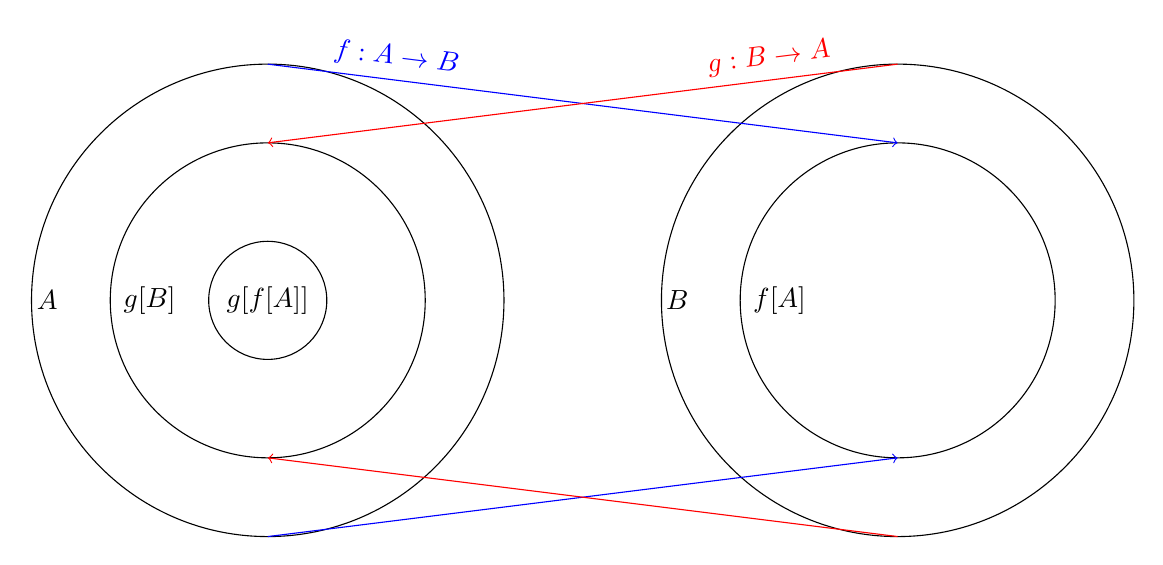
\begin{tikzpicture}
			\draw (-4, 0) circle (3); \draw (-6.8, 0) node {$A$};
			\draw (-4, 0) circle (2); \draw (-5.5, 0) node {$g[B]$};
			\draw (-4, 0) circle (0.75); \draw (-4, 0) node {$g[f[A]]$};
			
			\draw (4, 0) circle (3); \draw (1.2, 0) node {$B$};
			\draw (4, 0) circle (2); \draw (2.5, 0) node {$f[A]$};
			
			
			\draw[->, thin, blue] (-4, 3) -- (4, 2) node[pos=0.2, sloped, above, blue] {$f: A\to B$};
			\draw[->, thin, blue] (-4, -3) -- (4, -2);
			
			\draw[->, thin, red] (4, 3) -- (-4, 2)  node[pos=0.2, sloped, above, red] {$g:B\to A$};
			\draw[->, thin, red] (4, -3) -- (-4, -2);
			
		\end{tikzpicture}
	\end{center}
	\caption{Grafik des Sachverhalts im Satz \ref{SatzCantorSchroederBernstein}}
	\label{CantorSchroederBernsteinGrafik}
\end{figure}


\subsection{Ordinalzahlen}

Es wurden bereits die Zahlen $0,1,2,\dots,n,\dots,\omega,\omega+1,\omega+2,\dots,\omega+\omega$ diskutiert, mit welchen sich in diesem Kapitel genauer befasst werden soll.

Ein \textit{Graph} ist ein Paar $(A, R)$ so, dass $R\subseteq A\times A$ ein binäre Relation ist.

\begin{definition}[Partielle Ordnungen]
	Eine \textit{partielle Ordnung} ist ein Graph $(A,<)$ so, dass $<$ irreflexiv und transitiv ist. Eine alternative Definition ist $(A,\leq)$, wobei $\leq$ reflexiv, transitiv und antisymmetrisch ist.
\end{definition}

Eine \textit{lineare Ordnung} $(A,<)$ ist eine partielle Ordnung so, dass für alle $a,b\in A$ entweder $a<b$, $a=b$ oder $b<a$ gilt.

Ein Graph $(A,R)$ ist \textit{fundiert}, wenn jede nicht-leere Teilmenge $B\subseteq A$ ein Element $b\in B$ enthält so, dass $\{a\in B : (a,b) \in R\}= \emptyset$.
Also: Eine partielle Ordnung ist fundiert, wenn jede nicht-leere Teilmenge $B\subseteq A$ ein $<$-minimales Element enthält.

\begin{definition}[Wohlordnungen]
	Eine \textit{Wohlordnung} $(A,<)$ ist eine fundierte lineare Ordnung so, dass für jedes $a\in A$ die Klasse $\downarrow a\coloneqq \{b\in A : b < a\}$ eine Menge ist.
	Eine Relation $R\subseteq A\times A$, bei der für ein beliebiges $b$ die Klasse $\{a\in A : (a,b)\in R\}$ eine Menge ist wird auch als mengenähnlich bezeichnet.
\end{definition}

\begin{lemma}
	Sei $(A,<)$ eine fundierte, mengenähnliche, partielle Ordnung. Dann existiert in $A$ keine unendliche absteigende Folge $(a_n)_{n\in \omega}$ mit $a_{n+1}<a_n$ für alle $n$, wobei $\omega$ die Menge der natürlichen Zahlen bezeichnet.
\end{lemma}

Bemerkung: $(a_n)_{n\in \omega}$, $f:\omega \to A$ mit $a_n\coloneqq f(n)$

\begin{proof}
	Wenn eine solche Folge existiert, dann ist $\{a_n : n\in \omega\}=f[\omega]\subseteq A$ eine nicht-leere Klasse ohne $<$-minimales Element. Da $f[w]\subseteq \{a_0\}\cup \downarrow a$ und $A$ mengenähnlich ist, ist $f[w]$ eine Menge. Dies ist aber ein Widerspruch zur Fundiertheit.
\end{proof}

Um zu zeigen, dass jedes Element einer fundierten, mengenähnlichen partiellen Ordnung $(A,<)$ eine Eigenschaft $\psi$ erfüllt zeigt man, dass für für jedes $a$, dass wenn $\psi$ für alle $b<a$ gilt, dann auch für $a$.

\begin{satz}[Induktionsprinzip]
	Sei $(A,<)$ eine fundierte, mengenähnliche partielle Ordnung. Dann gilt
	\begin{itemize}
		\item[a)] Jede nicht-leere Klasse hat ein $<$-minimales Element.
		\item[b)] Sei $X\subseteq A$ so, dass für alle $a\in A$ gilt: Wenn $\downarrow a \subseteq X$, dann ist $a\in X$. Es folgt, dass $X=A$.
	\end{itemize}
\end{satz}
\begin{proof}
	a): Sei $B\subset A, a\in B$. Wegen der Mengenähnlichkeit ist $\downarrow a$ eine Menge und aus dem Aussonderungsaxiom folgt, dass auch $X\coloneqq B \cap (\downarrow a \cup \{a\})$ eine nicht-leere Teil\textit{menge} von $A$ ist. Es folgt auch, dass $X$ ein minimales Element $b$ besitzt. 
	
	Behauptung: $b$ ist auch das $<$-minimale Element von $B$. Andernfalls gibt es ein $c\in B$ mit $c < b \leq a$. Da $b\in X \subseteq B$ würde aber auch $c\in X$ folgen. Widerspruch!
	
	b): Annahme: $X$ sei wie gefordert, aber $X\neq A$. Also existiert ein $a\in A\setminus X$. Definiere $B\coloneqq \downarrow a \cup \{a\} \setminus \{X\}$. Dies ist eine nicht-leere Teilmenge und hat daher ein minimales Element $b$. Also ist $\downarrow b\subseteq A\setminus B\subseteq X$ und daher ist $b\in X$. Widerspruch!
\end{proof}

\begin{definition}[Ordinalzahlen]
	Eine \textit{Ordinalzahl} ist eine transitive Menge, welche durch $\in$ linear geordnet ist. 
	Beispiele sind $[n]$ für beliebige $n$, $\omega$, $\omega \cup \{\omega\}$. Die Klasse aller Ordinalzahlen ist $On$
\end{definition}

\begin{lemma}
	Ordinalzahlen sind wohlgeordnet durch $\in$.
\end{lemma}
\begin{proof}
	Sei $\beta\subseteq \alpha\in On$ und $\beta\neq \emptyset$. Da $\beta$ fundiert ist existiert ein $\gamma\in \beta$ mit $\gamma\cap \beta =\neq$. Also ist $\gamma$ kleinstes Element in $\beta$ bezüglich. $\in$
\end{proof}

\begin{definition}[Anfangsstück]
	Ein \textit{Anfangsstück} einer Ordnung $(A,<)$ ist eine Teilmenge $I\subseteq A$ so, dass, wenn $a\in I$ und $b<a$, auch $b\in I$ ist.
\end{definition}

Ein Anfangsstück von $\alpha \in On$ ist also eine Teilmenge $\beta\subseteq \alpha$ so, dass $\delta\in\gamma\in \beta\Rightarrow \delta\in\beta$, also eine transitive Teilmenge von $\alpha$.

\begin{lemma}
	Sei $\alpha\in On$. $\beta$ ist ein echtes Anfangsstück von $\alpha$, genau dann wen $\beta \in \alpha$
\end{lemma}
\begin{proof}
	\begin{itemize}
		\item[$\Rightarrow$:] Sei $\gamma$ das kleinste Element von $\alpha\setminus \beta$. 
		Es gilt $\beta=\gamma\in \alpha$, da für beliebige $\delta$ gilt, dass $\delta\in\gamma \Leftrightarrow (\delta\in\alpha \land \delta\notin\alpha\setminus\beta) \Leftrightarrow \delta\in\beta$
		\item[$\Leftarrow$:] Sei $\beta\in\alpha$ und $\delta\in\gamma\in\beta$. Es gilt $\delta\in\beta$, da sonst $\delta=\beta$ oder $\beta\in\delta$. Widerspruch!
	\end{itemize}
\end{proof}

\begin{satz}
	\begin{itemize}
		\item[a)] $(On,\in)$ ist ein Wohlordnung
		\item[b)] Wenn $\alpha\in On$, dann ist $\alpha=\{\beta\in On:\beta\in\alpha\}=\downarrow a$
		\item[c)] $On$ ist eine echte Klasse
	\end{itemize}
\end{satz}
\begin{proof}
	\begin{itemize}
		\item[a)] Zu zeigen ist, dass $\in$ eine lineare Ordnung ist. $\alpha \notin \alpha$ und $\alpha\in\beta, \beta\in \gamma\Rightarrow \alpha\in\gamma$ folgt direkt aus der Definition der Ordinalzahlen.
		
		Seien nun $\alpha,\beta\in On, \alpha\neq\beta$. Nun ist $x\in\alpha\cap\beta$ ein Anfangsstück von $\alpha$ und $\beta$. 
		Aus $y\in z \in \alpha\cap \beta$ folgt wegen der Transitivität $y\in\alpha\cap \beta$. Nun muss $x=\alpha$ oder $x=\beta$ gelten. Sonst ist $x\in \alpha$ und $x\in\beta$, also $\alpha\cap\beta \in \alpha\cap\beta$. Widerspruch!
		
		Wenn $x\in\alpha$, dann ist $x\in\beta$, also $\alpha \in \beta$, oder umgekehrt.
		
		\item[b)] Dies folgt direkt aus \textit{a)}
		
		\item[c)] Wäre $On$ eine Menge, wäre sie eine transitive, durch $\in$ linear geordnete Menge und müsste sich dadurch selbst enthalten. Widerspruch!
	\end{itemize}
\end{proof}

\begin{definition}[Nachfolgerordinal]
	Für $\alpha\in On$ ist $\alpha+1\coloneqq\alpha\cup \{\alpha\}$ das \textit{Nachfolgerordinal} von $\alpha$.
\end{definition}

\begin{definition}[Limesordinal]
	$\alpha\in On$ ist ein \textit{Limesordinal}, wenn $\alpha\neq\emptyset$ und $\alpha$ kein Nachfolgerordinal ist.
\end{definition}

Da $(On,\in)$, bzw. $(On,<)$, eine Wohlordnung ist, existiert die transfinite Induktion über $On$. Das heißt: für jede Teilklasse $X\subseteq On$ gilt: wenn für alle $\alpha\in On$ gilt, dass für jedes $\beta<\alpha$ aus $\beta\in X$ folgt, dass $\alpha\in X$, dann ist $X=On$.

Um zu zeigen, dass irgendeine Eigenschaft $\phi(x)$ aus alle Ordinale zutrifft, also $X\coloneqq\{\alpha\in On : \phi(x)\}=On$ gibt es folgende Strategien.
\begin{enumerate}
	\item Zeige, dass $\phi(0)$ gilt. Zeige, dass wenn $\phi(\alpha)$ auch $\phi(\alpha+1)$ ist. Zeige für jedes Limesordinal $\lambda$, dass $\phi(/lambda)$ gilt, wenn für alle $\alpha<\lambda$ auch $\phi(\alpha)$ korrekt ist.
	
	\item Betrachte eine beliebige Ordinalzahl $\alpha$ und nimm an, dass $\phi(\beta)$ für alle $\beta<\alpha$ gilt. Zeige, dass dann $\phi(\alpha)$ folgt.
\end{enumerate}

\subsubsection{Ordinale und Stufen}

Zur Erinnerung: für jede Menge $a$ ist $S(a)$ die kleinste Stufe mit $a\subseteq S(a)$ und aus $a\in b$ folgt $S(a)\in S(b)$.

Letzteres gilt natürlich auch für Ordinalzahlen. Wir wollen nun aber auch die Umkehrung betrachten. Wenn $\alpha\notin\beta$ ist, dann folgt $\alpha=\beta$ oder $\beta\in\alpha$, also $S(\alpha)=S(\beta)$ oder $S(\beta)\in S(\alpha)$. In beiden Fällen gilt $S(\alpha)\notin S(\beta)$. Es gilt also auch die Rückrichtung: $\alpha\in\beta \Leftrightarrow S(\alpha)\in S(\beta)$.

\begin{satz}
	Die Funktion $F:On \to H(\mathcal{S}), F(\alpha)\coloneqq S(\alpha)$ ist ein Isomorphismus zwischen $On$ und $H(\mathcal{S})$. Das heißt $F$ ist bijektiv und $\beta<\alpha \Leftrightarrow F(\beta)\in F(\alpha)$.
\end{satz}

Bemerkung: Mit $H(\mathcal{S})$ wird die Klasse aller Stufen, die Mengen sind, also aller Stufen außer $\mathcal{S}$ bezeichnet.

\begin{proof}
	Es ist bereits bekannt, dass $F$ injektiv und ein starker Homomorphismus ist. Es bleibt die Surjektivität zu beweisen. Wenn dies nicht der Fall wäre, dann existierte eine minimale Stufe $S\in\mathcal{S}$ mit $S\notin Bild(F)$. 
	
	Sei $X\coloneqq\{\beta\in On:S(\beta)\in S\}$. $X$ ist ein echtes Anfangsstück von $On$, das heißt es gibt $\alpha\in On$ so, dass $X=\downarrow \alpha=\alpha$. Demnach betrachten wir nun $S(\alpha)$ und wie sich dies zu $S$ verhält.
	\begin{itemize}
		\item $S(\alpha)\in S$, dann ist $\alpha\in X=\alpha$. Widerspruch!
		\item $S(\alpha)=S$, dann ist $S\in Bild(F)$. Widerspruch!
		\item $S\in S(\alpha)$, dann ist $S(\alpha)$ die kleinste Stufe so, dass $\alpha\subseteq S(\alpha)$, sodass $\beta\in S(\alpha)$ für alle $\beta\in\alpha$ gilt. 
		Da aber $\beta\in S(\beta)\in S$ für alle $\beta\in\alpha$ ist, folgt $S(\alpha)\subseteq S$. Widerspruch!
	\end{itemize}
\end{proof}

\begin{definition}
	Für $\alpha\in On$, setze $S_\alpha\coloneqq S(\alpha)$. Dies sind dann die \textit{Indices der kumulativen Hierarchie}.
\end{definition}

Es folgt, dass $S_0\subset S_1 \subset \dots \subset S_\omega \subset \dots \subset S_\alpha \subset S_{\alpha+1}\subset\dots$, $H(\mathcal{S})=\{S_\alpha:\alpha\in On\}$ und $\mathcal{S}=\bigcup\{S_\alpha : \alpha\in On\}$.

\begin{definition}[Rang einer Menge]
	Der \textit{Rang} einer Menge $a$ ist das Ordinal $\rho(a)=\alpha$ mit $S(a)=S_\alpha$.
\end{definition}

Für Ordinale $\alpha$ gilt $\rho(\alpha)=\alpha$. Eine Klasse $X$ ist eine Menge genau dann, wenn $\{\rho(x):x\in X\}$ durch eine Ordinalzahl beschränkt ist.

\subsubsection{Der Rekursionssatz}

Sei $A$ eine Klasse und definiere $A^\infty\coloneqq\{f : f:\alpha\to A, \text{Fkt. für ein} \alpha\in On\}$. Dies lässt sich in Worten als die Menge aller Folgern der Länge $\alpha$.

Sei $G$ nun eine partielle Funktion $G:\mathcal{S}^\infty\to\mathcal{S}$.

\begin{lemma}
	Es gibt höchstens eine Funktion $f:\alpha\to \mathcal{S}$ so, dass $f$ eine Menge ist und $f(\beta)=G(f\upharpoonright\beta)$ für alle $\beta < \alpha$.
\end{lemma}
Bsp.: $f(17)=G(f\upharpoonright\{0,\dots,16\})$.
\begin{proof}
	Nehmen wir an, dass $f$ und $f'$ die geforderte Eigenschaft erfüllen. Sei $X=\{\beta \in\alpha : f(\beta)=f'(\beta)\}$. Wenn $\beta < \alpha$ und $\beta\subseteq X$, dann $f\upharpoonright\beta =f'\upharpoonright\beta$, also $f(\beta)=G(f\upharpoonright\beta)=G(f'\upharpoonright\beta)=f'(\beta)$, also $\beta\in X$. Es folgt $X=\alpha$ und $f=f'$.
\end{proof}

Nun ist das Ziel zu zeigen, dass jede totale Funktion $G:\mathcal{S}^\infty\to\mathcal{S}$ auf eindeutige Weise eine Funktion $F:On\to\mathcal{S}$ definiert.

Für die Existenz wird aber ein zusätzliches Axiom benötigt:

\textit{Ersetzungsaxiom}: Wenn $F:A\to S$ eine Funktion ist und $a\subseteq A$ eine Menge ist, dann ist auch $F[a]$ eine Menge. Oder in anderen Worten: Wenn $F$ eine Funktion ist und $Def(F)$ eine Menge ist, dann ist auch $Bild(F)$ eine Menge.

\begin{satz}[Rekursionssatz]
	Zu jeder Funktion $G:\mathcal{S}^\infty\to\mathcal{S}$ gibt es genau eine Funktion $F:On\to\mathcal{S}$ so, dass $F(\alpha)=G(F\upharpoonright\alpha)$ für alle $\alpha\in On$.
\end{satz}
\begin{proof}
	Sei $\alpha\in On$. Wir wissen dass es höchstens eine Funktion $f_\alpha:\alpha\to\mathcal{S}$ mit $f_\alpha(\beta)=G(f\alpha\upharpoonright\beta)$ für alle $\beta<\alpha$ gibt.
	
	Die Existenz solch einer Funktion $f_\alpha$ soll nun per Induktion nach $\alpha$ geschehen so, dass für alle $\beta<\alpha$ gilt, dass $f_\beta=f_\alpha\upharpoonright\beta$.
	
	$\alpha=0$: Dann ist $f_\alpha=\emptyset$, die Bedingung gilt also.
	
	$\alpha+1$: Dann lässt sich $f_{\alpha+1}$ als $f_{\alpha+1}\coloneqq f_\alpha\cup\{(\alpha, F(f_\alpha))\}$ definieren.
	
	Sei $\alpha$ ein Limesordinal. Setze $X\coloneqq\{f_\beta : \beta < \alpha\}$. $X$ ist eine Menge, denn $X$ ist das Bild der Funktion $H:\alpha\to\mathcal{S}^\infty$ mit $H(\beta)=f_\beta$ für $\beta\in\alpha$.
	
	Nun ist $f_\alpha\coloneqq\bigcup X=\{(\gamma,f_\beta(\gamma), \gamma<\beta<\alpha)\}$. $f_\alpha$ ist tatsächlich eine Funktion von $\alpha$ nach $\mathcal{S}$: Für alle $\gamma<\alpha$ existiert ein $\beta$ mit $\gamma<\beta<\alpha$ und damit ein Paar $(\gamma,f_\beta(\gamma))\in f_\alpha$. Für $(\gamma,f_\beta(\gamma)),(\gamma,f_{\beta'}(\gamma))\in f_\alpha$ so, dass $\beta<\beta'$ ist $f_\beta=f_{\beta'}\upharpoonright \beta$, also $f_\beta(\gamma)=f_{\gamma'}(\gamma)$. Es folgt also $Def(f_\alpha)=\alpha$.
	
	Setze $F=\bigcup\{f_\alpha:\alpha\to\mathcal{S} : \alpha\in On\}$. $F=\{(\beta, f_\alpha(\beta)):\beta<\alpha\in On\}$, $F$ ist eine Funktion mit $Def(F)=On$.
	
	Für jedes $\beta\in On$ ist $F(\beta)=f_\alpha(\beta)$ für ein (und damit alle!) $\alpha$ mit $\beta<\alpha$.
	
	$F\upharpoonright\beta=f_\alpha\upharpoonright\beta$ für $\beta<\alpha$, $F(\beta)=f_\alpha(\beta)=G(f_\alpha\upharpoonright\beta)=G(F\upharpoonright\beta)$.
\end{proof}

Damit ist der Rekursionssatz bewiesen. Nun sollen Anwendungen von diesem gezeigt werden.\\

\textit{Konstruktion von $F:On\to A$}: Sei $a\in A,s:A\to A, h: \Pot{A}\to A$. Nun lässt sich $G:A^\infty\to A$ definieren durch: $G(\emptyset)\coloneqq a, G(F\upharpoonright\alpha+1)\coloneqq s(F(\alpha)), G(F\upharpoonright\lambda)\coloneqq h(F[\lambda])$ für ein Limesordinal $\lambda$ und Nachfolgerordinal $\alpha$.

Mit dem Rekursionssatz folgt die Existenz und Eindeutigkeit der Funktion $F:On\to A$ mit $F(\alpha)=F(F\upharpoonright\alpha)$. Es gilt $F(\emptyset)=a, F(\alpha+1)=s(F(\alpha)), F(\lambda)=h(F[\lambda])$.\\

\textit{Addition von Ordinalzahlen}: Es sollen nun Ausdrücke wie $\alpha+\beta$ definiert werden, für $\alpha,\beta\in On$. $\alpha+\beta\coloneqq F_\alpha:On\to On, \beta\mapsto\alpha+\beta$. 
Genauer lässt sich rekursiv definieren, dass 
\begin{align*}
	&\alpha+0\coloneqq\alpha,\\
	&\alpha+(\beta+1)\coloneqq(\alpha+\beta)+1,\\ 
	&\alpha+\lambda\coloneqq\sup\{\alpha+\beta : \beta < \alpha\}
\end{align*}
für ein Limesordinal $\lambda$.

\textit{Bemerkung}: Addition ist nicht kommutativ! Dies lässt sich leicht an einem Beispiel erkennen: $\omega+1=\omega\cup\{\omega\}\neq\omega$, aber $1+\omega=\sup\{1+n:n\in\omega\}=\omega$.

Eine andere interessante Beobachtung ist, dass sich Addition zweier Ordinalzahlen durch \glqq Hintereinanderlegen\grqq{} zweier Wohlordnungen darstellen lässt. Für $\alpha+\beta$ lassen sich Strukturen $\mathfrak{A}=(A,<), \mathfrak{B}=(B,<)$ finden, wobei beide Strukturen Wohlordnungen sind. Das \glqq Hintereinanderlegen\grqq{} lässt sich in Abbildung \ref{AdditionWO} erkennen. Da $\mathfrak{A}$ und $\mathfrak{B}$ beides Wohlordnungen sind, lässt sich leicht einsehen, dass dann auch $\mathfrak{A}+\mathfrak{B}$ eine Wohlordnung ist.
	
\begin{figure}[h]
	\begin{center}
		\begin{tikzpicture}
			\draw (-5, 0) node {$\mathfrak{A}+\mathfrak{B}$:};
	
			\draw[-{Latex}, thin] (-4, 0) -- (-0.05, 0) node[midway, below] {$(A,<)$};		
			\draw[-{Latex}, thin] (0.05, 0) -- (4, 0) node[midway, below] {$(B,<)$};
		\end{tikzpicture}
	\end{center}
	\caption{Darstellung von Addition durch \glqq Hintereinanderlegen\grqq{} von Wohlordnungen}
	\label{AdditionWO}
\end{figure}

\textit{Multiplikation von Ordinalzahlen}: Analog zur Addition kann man auch die Multiplikation definieren. Für $\alpha,\beta\in On$ ist dafür definiert:
\begin{align*}
	&\alpha\cdot0\coloneqq 0\\
	&\alpha\cdot(\beta+1)\coloneqq\alpha\cdot\beta+\alpha\\
	&\alpha\cdot\lambda\coloneqq\sup\{\alpha\cdot\beta : \beta<\lambda\}
\end{align*}
für ein Limesordinal $\lambda$.

Und ebenso, wie Addition durch Wohlordnungen darstellbar ist, lässt sich Multiplikation mithilfe von zwei Wohlordnungen $\mathfrak{A}=(A,<)$ und $\mathfrak{B}=(B,<)$ bilden. Dabei gilt $\mathfrak{A}\cdot\mathfrak{B}\coloneqq\mathfrak{C}=(A\times B, <_C)$ mit $(a,b)<_C(a',b')$ genau dann, wenn $b<b'$ oder $b=b'\land a<a'$. Graphisch dargestellt ist dies in Abbildung \ref{MultiplikationWO}.
	
\begin{figure}[h]
	\begin{center}
		\begin{tikzpicture}
			\draw[-{Latex}, thin] (-5, 0) -- (-1, 0) node[midway, below] {$\mathfrak{A}$};
			
			\draw (-0.5, 0) node[very thick] {$\cdot$};
			
			\draw[-{Latex}, thin] (0, -2) -- (0, 2) node[midway, right] {$\mathfrak{B}$};
			
			\draw (1, 0) node[very thick] {$=$};
			
			\draw[-{Latex}, thin] (1.5, -2) -- (1.5, 2);
			
			% Top (y=2)
			\draw[-{Latex}, thin] (1.7, 1.7) -- (5.7, 1.7);
			
			% Upper (y=1)
			\draw[-{Latex}, thin] (1.7, 0.85) -- (5.7, 0.85);
			
			% Middle (y=0)
			\draw (3.7, 0) node[very thick] {$\vdots$};
			
			% Lower (y=-1)
			\draw[-{Latex}, thin] (1.7, -0.85) -- (5.7, -0.85);
			
			% Bottom (y=-2)
			\draw[-{Latex}, thin] (1.7, -1.7) -- (5.7, -1.7);
			
		\end{tikzpicture}
	\end{center}
	\caption{Graphische Darstellung von Multiplikation mithilfe von Wohlordnungen}
	\label{MultiplikationWO}
\end{figure}

Auch hier lässt es sich wieder feststellen, dass Multiplikation nicht kommutativ ist. Ein Beispiel hierfür ist $\omega\cdot 2=\omega\cdot(1+1)=\omega+\omega=\sup\{\omega+n : n\in\omega\}>\omega+n$ für alle $n\in\omega$, aber $2\cdot\omega=\sup\{2\cdot n : n<\omega\}=\omega<\omega+1$.

Also gilt im Allgemeinen auch \textbf{nicht} $(\alpha+\alpha')\cdot\beta=\alpha\beta+\alpha'\beta$, da beispielsweise $(1+1)\cdot\omega=2\cdot\omega=\omega \neq \omega+\omega = 1\cdot\omega+1\cdot\omega$.\\

\textit{Potenzen von Ordinalzahlen}: Zuletzt wird nun noch das Potenzieren von Ordinalzahlen definiert. Für $\alpha,\beta,\lambda\in On$, $\alpha, \beta$ Nachfolgerordinale und $\lambda$ ein Limesordinal sein nun definiert:
\begin{align*}
	&\alpha^0\coloneqq1\\
	&\alpha^{\beta+1}\coloneqq\alpha^\beta\cdot\alpha\\
	&\alpha^\lambda\coloneqq\sup\{\alpha^\beta:\beta<\lambda\}.
\end{align*}

\begin{satz}[Cantor-Normalform]
	Jedes $\alpha\in On$ hat eine eindeutige Darstellung $\alpha=\omega^{\beta_1}\cdot n_1+\dots+\omega^{\beta_k}\cdot n_k$ mit $k\in\omega, n_1,\dots, n_k\in\omega\setminus\{0\}$ und $\alpha\geq\beta_1>\beta_2>\dots>\beta_k\geq0$.
\end{satz}
\begin{proof}
	Dies soll per Induktion gezeigt werden. Für $\alpha=0$ ist dies trivial, da dies die einzige Darstellung der $0$ ist. Sei unsere Induktionsvoraussetzung nun also, dass alle Ordinale, die kleiner als $\alpha$ sind eine eindeutige Cantor-NF besitzen.
	
	Sei $\gamma$ das kleinste Ordinal so, dass $\omega^\gamma>\alpha$. $\gamma$ muss ein Nachfolger sein, denn wäre es ein Limesordinal, dann wäre $\gamma$ nicht das kleinste Ordinal mit der geforderten Eigenschaft.
	
	Also ist $\gamma=\beta+1$ und $\beta$ ist das größte Ordinal mit $\omega^\beta \leq \alpha$. Also existieren Ordinale $n<\omega$ und $\gamma$ so, dass $\alpha=\omega^\beta\cdot n+\gamma, \gamma<\omega^\beta\leq\alpha$.
	
	Nach der Induktionsvoraussetzung hat $\gamma$ eine eindeutige Cantor-Normalform und damit auch $\alpha$.
\end{proof}

Es lässt sich jedoch feststellen, dass die Cantor-NF nicht immer hilfreich ist. Sei beispielsweise $\omega_1=\min\{\alpha\in On : \text{ es gibt keine injektive Abb.} f:\alpha\to\omega\}$ das kleinste nicht abzählbare Ordinal. Gesucht sei nun die Cantor-Normalform von $\omega_1$.

$\omega_1=\sup\{\alpha\in On : \alpha \text{ ist abzählbar}\}$ ist ein Limesordinal. Betrachte nun $\omega^{\omega_1}=\sup\{\omega^\alpha : \alpha \text{ ist abzählbar}\}$. Es lässt sich feststellen, dass $\omega^{\omega_1}\leq\omega_1\leq\omega^{\omega_1}$, also muss $\omega_1=\omega^{\omega_1}$ sein.

Die Cantor-NF von $\omega_1$ ist also $\omega^{\omega_1}$, was offensichtlicherweise nicht sonderlich hilfreich ist.

\begin{satz}[Ordinale Normalform für Wohlordnungen]
	Jede Wohlordnung $(a,<)$ über einer Menge $a$ ist isomorph zu genau einer Ordinalzahl.
\end{satz}
\begin{proof}
	Zu einer gegebenen Wohlordnung $(a,<)$ suchen wir ein $\alpha\in On$ und eine bijektive Abbildung $f:\alpha\to a$ so, dass für $\gamma<\beta<\alpha$ auch $f(\gamma)<f(\beta)$ ist.
	
	Definiere $F:On\to a\cup\{a\}$ durch
	$$
	F(\alpha)\coloneqq\begin{cases}
		\min\{a\setminus F[\alpha]\} & \text{wenn } F[\alpha]\subsetneqq a\\
		a & \text{sonst}
	\end{cases}
	$$
	
	Behauptung: $a\in Bild(F)$. Andernfalls wäre $F$ eine injektive Abbildung von $On$ nach $a$, dann wäre für $\beta<\alpha$ aber entweder $F(\alpha)\notin F[\alpha]$ oder $F(\beta)\in F[\alpha]$, also $F(a)\neq F(b)$. Das heißt, dass $F:On\to Bild(F)$ bijektiv ist und da $Bild(F)\subseteq a$ eine Menge ist, müsste $F^{-1}[Bild(F)]=On$ nach dem Ersetzungsaxiom eine Menge sein. Widerspruch!
	
	Sei $\alpha$ also die kleinste Ordinalzahl so, dass $F(\alpha)=a$. Dann ist $f:F\upharpoonright \alpha$ die gesuchte Bijektion:
	\begin{itemize}
		\item $f$ ist Ordnungserhaltend und damit auch injektiv, da für $\gamma<\beta<\alpha$ folgt, dass $f[\gamma]\subsetneqq f[\beta]$, da $f(\gamma)=\min\{a\setminus f[\gamma]\}<\min\{a\setminus f[\beta]\}=f(\beta)$.
		\item $f$ ist surjektiv, da sonst ein kleinstes Element $b\in a\setminus f[\alpha]$ existieren würde. Dann wäre $F(\alpha)=b$ im Widerspruch zu $F(\alpha)=a$.
	\end{itemize}
\end{proof}

\subsection{Das Auswahlaxiom (AC)}

\begin{definition}[Auswahlfunktionen]
	Eine \textit{Auswahlfunktion} auf einer Menge $x$ ist eine Funktion $f:x\to\mathcal{S}$ so, dass $f(z)\in z$ für jedes nicht-leere $z\in x$.
\end{definition}

Das Auswahlaxiom (AC) besagt, dass auf jeder Menge eine solche Auswahlfunktion existiert.\\

Es lässt sich sehen, dass wenn auf $\bigcup X$ eine Wohlordnung existiert, man eine Auswahlfunktion bilden kann, ohne das Auswahlaxiom nutzen zu müssen. Sei $z\in x, z\neq\emptyset$. Dann ist $f(z)=\min(z)$ eine Auswahlfunktion. 

Dies ist die eine Richtung des Wohlordnungssatzes von Zermelo, welches auch aus dem AC folgt. Die andere Richtung soll nun ebenfalls gezeigt werden.

\begin{satz}[Wohlordnungssatz von Zermelo]
	Auf jeder Menge $a$ existiert eine Wohlordnung.
\end{satz}
\begin{proof}
	Aus einer Auswahlfunktion $f$ auf $\Pot{a}$ können wir eine Wohlordnung auf $a$ konstruieren. Sei $F:On\to a\cup \{a\}$ mit
	$$
	F(\alpha)=\begin{cases}
		f(a\setminus F[\alpha]) & \text{wenn } F[\alpha]\subsetneqq a \\
		a & \text{sonst}
	\end{cases}
	$$
	Wie im letzten Beweis gezeigt gibt es ein $\alpha\in On$ mit $F(\alpha)=a$ und $F\upharpoonright \alpha:\alpha\to a$ bijektiv.
	
	$F\upharpoonright\alpha$ ist surjektiv, denn sonst ist $F(\alpha)\neq a$ und $F\upharpoonright\alpha$ überträgt de Wohlordnung von $\alpha$ auf $a$. Für $y,z\in a$ setze $y <_a z$ genau dann, wenn $(F\upharpoonright\alpha)^{-1}(y) < (F\upharpoonright\alpha)^{-1}(z)$.
\end{proof}

Ein weiteres, zum Auswahlaxiom äquivalentes Axiom ist das Lemma von Zorn (Kuratowski).
Dieses besagt, dass wenn $(a,<)$ eine partielle Ordnung auf einer Menge $a$ ist, in der jede linear geordnete Teilmenge $b\subseteq a$ eine obere Schranke $s_b\in a$ hat, die Menge ein maximales (bemerke: nicht größtes) Element $m_a$ besitzt.

\begin{satz}
	Aus den Axiomen von ZF und dem Auswahlaxiom lässt sich das Lemma von Zorn folgern.
\end{satz}
\begin{proof}
	Sei $f$ eine Auswahlfunktion auf $\Pot(a)$. Für jede Teilmenge $b\subseteq a$, welche durch $<$ linear geordnet ist, setze $y_b\coloneqq\{x\in a:\forall u(u\in b\rightarrow u<x)\}$ als die Menge der \textit{echten} oberen Schranken von $b$.
	
	Definiere nun $F:\Pot{a}\to a\cup\{a\}$ durch
	$$
	F(b)\coloneqq\begin{cases}
		f(y_b) & \text{wenn } b \text{ durch } < \text{ linear geordnet ist und } y_b\neq\emptyset \\
		a & \text{sonst}
	\end{cases}
	$$
	
	Mithilfe des Rekursionssatzes lässt sich dann eine Funktion $G: On\to a\cup\{a\}$ mit $\alpha\mapsto G(G[\alpha])=F(Bild(G\upharpoonright\alpha))$ definieren.
	
	$G[\alpha]$ ist eine linear geordnete Teilmenge von $a$ und $G(\alpha)$ ist eine echte obere Schranke für $G[\alpha]$ außer dann, wenn $G[\alpha]$ keine echte obere Schranke besitzt, dann gilt $G(\alpha)=a$.
	
	Wie in vorherigen Beweisen folgt, dass $G$ den Wert $a$ annehmen muss, da sonst $G$ eine ordnungserhaltende Abbildung von $On$ nach $a$ wäre und $On$ eine Menge sein würde.
	
	Sei $\alpha$ also minimal mit $G(\alpha)=a$. $G[\alpha]$ ist nach Konstruktion eine linear geordnete Teilmenge von $a$ ohne \textit{echte} obere Schranke.
	
	Sei $m$ eine obere Schranke (und damit größtes Element) von $G[\alpha]$. Damit ist $m$ maximales Element von $(a,y)$.
\end{proof}

\begin{satz}
	Aus den Axiomen von ZF und dem Lemma von Zorn folgt das Auswahlaxiom.
\end{satz}
\begin{proof}
	Sei $x$ eine beliebige Menge und $a\coloneqq\{f:z\to\bigcup z : z\subseteq x \text{ und } f \text{ ist eine Auswahlfunktion auf } z\}$.
	Es gilt $a\neq\emptyset$, da die leere Funktion in $a$ ist und $a$ ist durch $\subsetneqq$ partiell geordnet.
	
	Wir behaupten, dass jede lineare geordnete Teilmenge $b\subseteq a$ eine obere Schranke $g_b\in a$ besitzt. Setze $g_b\coloneqq \bigcup b\subseteq x\times \bigcup x$, so dass $g_b=\{(c, f(c)) : c\in z\subseteq x, f:z\to\bigcup z, f\in b\}$. Wenn $(c,f(c)),(c,f'(c))\in g_b$ sind, dann ist $f, f'\in b$, aber es gilt $f\subseteq f'$ oder $f'\subseteq f$. Da $f,f'$ Funktionen sind, folgt $f(c)=f'(c)$, $g_b$ ist also eine wohldefinierte Funktion.
	
	Für $c\in Def(g_b)$ ist $g_b(c)=f(c)\in c$ für ein $f\in b$. Also ist $g_b$ eine Auswahlfunktion, das heißt $g_b\in a$.
	
	Schließlich ist $g_b$ eine obere Schranke für $b$, also besitzt $a$ nach dem Zornschen Lemma ein maximales Element $f\in a$.
	
	Behauptung: $f$ ist eine Auswahlfunktion auf $x$. Wenn nicht, dann ist $f$ eine Auswahlfunktion auf einer echten Teilmenge $z\subsetneqq x$ und es gibt ein nicht-leeres $y\in x\setminus z$. Für jedes $c\in y$ ist dann $f'\coloneqq f\cup\{(y,c)\}$ eine Auswahlfunktion auf $z\cup\{y\}\subseteq x$ mit $f\subsetneqq f'$. Widerspruch zur Maximalität von $f$.
\end{proof}

\subsubsection{Folgerungen aus dem Auswahlaxiom}

\begin{satz}
	Jeder Vektorraum hat eine Basis.
\end{satz}
\begin{proof}
	Sei $V$ ein Vektorraum. Wenn $V=\{0\}$, dann ist $\emptyset$ eine Basis. Sei also $V\neq\{0\}$. Definiere $X\coloneqq\{B\subseteq V : B\text{ ist unabhängig}\}$ (zur Erinnerung: $B\subseteq B$ ist unabhängig, wenn kein Element $v\in B$ sich als endliche Linearkombination von anderen Elementen aus $B$ schreiben lässt).
	
	$X$ ist nicht leer, da für $V\neq\{0\}, v\in V$ die Menge $\{v\}$ linear unabhängig ist.
	
	Weiter folgt, dass $(X,\subsetneqq)$ eine partielle Ordnung ist, in der jede Kette $K\subseteq X$ eine obere Schranke, nämlich $\bigcup K$ besitzt. Es gilt $\bigcup K\in X$, denn sonst lässt sich ein $v\in\bigcup K$ als endliche Linearkombination $v=\lambda_1v_1+\dots+\lambda_kv_k$ schreiben. Aber dann existiert ein $B\in K$ mit $v,v_1,\dots,v_m\in B$.
	
	Nach dem Lemma von Zorn hat $X$ also ein maximales Element $B_{max}$. $B_{max}$ ist unabhängig, jedes $v\in V$ lässt sich als Linearkombination $v=\lambda_1v_1+\dots+\lambda_mv_m$ schreiben. Sonst wäre $B_\{max\}\bigcup \{v\}$ unabhängig, im Widerspruch zur Maximalität von $B_{max}$.
\end{proof}

Eine weitere Folgerung des Auswahlaxioms ist der Satz von Banach-Tarski, welcher im folgenden Kapitel genauer betrachtet werden soll.

\subsubsection{Der Satz von Banach-Tarski}

Informell lässt sich der Satz wie folgt definieren: \glqq Eine Kugel $B\subseteq\mathbb{R}^3$ kann in endlich viele Teile zerlegt werden, die dann via einfacher Isometrien zu zwei disjunkten Kopien von $B$ zusammengesetzt werden können.\grqq{}

Im Folgenden werden nun einige begriffe definiert:

\begin{definition}[Isometrie]
	Sei $A\subseteq\mathbb{R}^3$. Eine Funktion $\phi:A\to\mathbb{R}^3$ ist eine \textit{Isometrie}, wenn $\Vert\phi(a)-\phi(b)\Vert=\Vert a-b\Vert$ für alle $a,b\in A$.
\end{definition}

\begin{definition}[Kongruenz]
	Zwei Mengen $A,B\subseteq\mathbb{R}^3$ sind \textit{kongruent} ($A\cong B$), wenn eine Isometrie $\varphi$ auf $A$ existiert mit $\varphi(A)=B$.
\end{definition}

\begin{definition}[Zerlegungsäquivalenz]
	$A, B$ sind \textit{Zerlegungsäquivalent} ($A\sim_z B$), wenn $n\in\mathbb{N}$ und Partitionen $A=A_1\cup\dots\cup A_n, B=B_1\cup\dots\cup B_n$ existieren, mit $A_i\cong B_i$ für alle $i\leq n$.
\end{definition}

Es bleibt nun zu zeigen, dass $\sim_z$ eine Äquivalenzrelation ist. Reflexivität und Symmetrie ist leicht einsehbar, gezeigt werden muss nun also nur noch die Transitivität.

Sei $A\sim_z B$ und $B\sim_z C$. Es gibt also Partitionen 
\begin{align*}
	&A=A_1\cup\dots\cup A_n,\\
	&B=B_1\cup\dots\cup B_n \text{ mit}\\
	&\varphi_i \text{ so, dass q} A_i\cong B_i, \forall i\leq n
\end{align*}
und 
\begin{align*}
	&B=B'_1\cup\dots\cup B'_m,\\
	&C=C_1\cup\dots\cup C_m \text{ mit}\\
	&\psi_i \text{ so, dass } B'_i\cong C_i, \forall i\leq m
\end{align*}

Setze $B_{ij}\coloneqq B_i\cap B'_j, i\leq n, j\leq m$, wodurch wieder eine Partition von $B$ gebildet wird. Weiter sei $A_{ij}\coloneqq\phi_i^{-1}(B_{ij})$ und $C_{ij}\coloneqq\psi_j(B_{ij})$.

Dann ist $\psi_j\circ\phi_i$ eine Isometrie von $A_{ij}$ nach $C_{ij}$ und $A_{ij}, C_{ij}$ bilden Partitionen von $A$ bzw. $C$, also ist $A\sim_z C$.

Weiter kann man folgende Eigenschaften der Relationen $\sim_z$ feststellen, welche hier aber nicht bewiesen werden sollen:
\begin{itemize}
	\item Wenn $A\sim_z B$, dann existiert eine Bijektion $g:A\to B$ mit $C\sim_z g(C)$ für alle $C\subseteq A$
	\item Für Partitionen $A=A_1\cup\dots\cup A_n, B=B_1\cup\dots\cup B_n$ mit $A_i\sim_z B_i$ folgt $A\sim_z B$.
	\item Wir definieren $A\leq B\colon\Leftrightarrow \exists B'\subseteq B : A\sim_z B'$
	\item Wenn $A\leq B$ und $B\leq A$, dann ist $A\sim_z B$
\end{itemize}

Ein Vorbereitender Satz für den Satz von Banach-Tarski ist das Hausdorff-Paradoxon. Dieses beschreibt eine Paradoxe Zerlegung der $2-$Sphäre $S^2=\{(x,y,z)\in\mathbb{R}^3 : x^2+y^2+z^2=1\}$.

\begin{satz}[Hausdorff-Paradoxon]
	Es gibt Mengen $A,B,C,D\subseteq S^2$ mit
	\begin{itemize}
		\item $A,B,C,D$ bilden eine Partition von $S^2$
		\item $D$ ist abzählbar
		\item $A\cong B \cong C \cong (B\cup C)$
	\end{itemize}
\end{satz}
\begin{proof}
	Definiere
	$$
	\psi\coloneqq
	\begin{pmatrix}
		-\frac{1}{2} & \frac{\sqrt{3}}{2} & 0 \\
		-\frac{\sqrt{3}}{2} & -\frac{1}{2} & 0 \\
		0 & 0 & 1 \\
	\end{pmatrix}
	$$
	als eine Rotation um $\frac{2\pi}{3}=120^\circ$, um die z-Achse (die z-Achse ist die Achse, die nach \glqq oben\grqq{} geht). Es gilt $\psi^3=1=id_{\mathbb{R}^3}$.
		
	Weiter sei 
	$$
	\varphi_\theta\coloneqq
	\begin{pmatrix}
		-\cos \theta & 0 & \sin \theta \\
		0 & -1 & 0 \\
		\sin \theta & 0 & \cos \theta 
	\end{pmatrix}
	$$
	eine Rotation um $\pi=180^\circ$, um die Achse $a_\theta$ in der x-z-Ebene (die x-z-Ebene ist die Ebene parallel zur Tafel in der Vorlesung). Hier gilt dann $\varphi_\theta\cdot\varphi_\theta=1$.
	
	Die Gruppe $(G_\theta, \cdot)$ lässt sich nun durch reduzierte Wörter $g=g_1\dots g_n$ über dem Alphabet $\Gamma=\{\psi, \psi^2,\phi\}$ darstellen so, dass hintereinander stehende Zeichen, welche sich zu $1$ kürzen nicht vorkommen. Die Darstellung ist also eindeutig.
	
	Wir wollen $\theta$ so wählen, dass $G_\theta$ frei ist, das heißt, dass für jedes $g\in G_\theta$ genau eine Darstellung $g=g_1\dots g_n$ durch ein reduziertes Wort existiert. Solche $\theta$ existieren.
	
	Für $g=g_1\dots g_n\in \Gamma^\ast$ sei $g(\theta)$ die Rotation die entsteht, wenn wir $\varphi=\varphi_\theta$ setzen. Und es sei $\theta_g\coloneqq\{\theta\in[0,2\pi) : g(\theta)=1\}$.
	
	\begin{lemma}
		Für jedes $g\in\Gamma^\ast\setminus\{\varepsilon\}$ ist $\theta_g$ endlich.
		\label{HausdorffOhneProof}
	\end{lemma}

	Mithilfe des Lemmas \ref{HausdorffOhneProof} lässt sich folgern, dass $M=\bigcup\limits_{g\in\Gamma^+, g\text{ red.}}\theta_g$ abzählbar ist und wir ein $\theta\in [0,2\pi]\setminus M$ finden können. Dann ist $g(\theta)\neq 1$ für alle reduzierten $g\in\Gamma^+$ und also $G_\theta$ frei über $\{\psi,\psi^2,\varphi_\theta\}$. Fixiere ein solches $\theta$ und sei $\varphi\coloneqq\varphi_\theta$ sowie $D\coloneqq\{s\in S^2 : gx=x\text{ für ein } g\in G_\theta\}$. Jede nicht-triviale Rotation fixiert genau zwei Punkte von $S^2$, die Schnittpunkte mit der Rotationsachse, also ist $D$ abzählbar
	
	Sei $Q\coloneqq S^2\setminus D$. Die Bahn von $x\in Q$ unter $G_\theta$ ist $G_\theta x=\{gx : g\in G_\theta\}$. Die Bahnen von $G_\theta$ auf $Q$ bilden eine Partition. Mit dem Auswahlaxiom existiert also eine Auswahlfunktion auf der Menge dieser Bahnen und damit eine Menge $R$, welche aus jeder Bahn $G_\theta x$ für $x\in Q$ genau ein Element enthält. Damit ist $Q=\bigcup\{gR : g\in G_\theta\}=\{gr : g\in\Gamma^\ast,r\in R\}$.
	
	Wir konstruieren die Zerlegung $Q=A\dot{\cup} B \dot{\cup}C$ induktiv gemäß der Länge von $g$. Wenn $\vert g \vert=0$, d.h. $g=1$ und $gr=r$, setzen wir $r\in A$, also ist $R\subseteq A$. Für $\vert g \vert = n+1$, also ist $gr=h\tilde{g}r$ mit $h\in\{\psi,\psi^2,\varphi\}$, definieren wir die Zugehörigkeit von $gr$ zu $A,B,C$ gemäß der Tabelle \ref{HausdorffTabelle}.
	\begin{table}[h]
		\begin{center}
			\begin{tabular}{c|ccc}
				$\tilde{g}h$ & $\varphi$ & $\psi$ & $\psi^2$ \\
				\hline
				$A$ & $B$ & $B$ & $C$ \\
				$B$ & $A$ & $C$ & $A$ \\
				$C$ & $A$ & $A$ & $B$ \\
			\end{tabular}
		\end{center}
		\caption{Tabelle für die Zugehörigkeiten zu den Mengen für das Hausdorff-Paradoxon}
		\label{HausdorffTabelle}
	\end{table}

	Da jedes Element von $Q$ eine eindeutige Darstellung $g\cdot r$ hat, ist damit die Partition $Q=\dot{\cup}B\dot{B}\dot{C}$ und damit $S^2=A\dot{\cup}B\dot{\cup}C\dot{\cup}D$ definiert. Es bleibt zu zeigen, dass $A\widetilde{=}B\widetilde{=}C\widetilde{=}B\cup C$ gilt. Wir behaupten, $\psi(A)=B$, $\psi^2(A)=C$ und $\varphi(A)=B\cup C$.
	\par
	
	$\psi(A)\subseteq B$: Sei $A=g\cdot r \in A$.
	\begin{itemize}
		\item Falls $g=\varphi\tilde{g}$, ist $\psi(a)=\psi\varphi\tilde{g}r\in B$ gemäß der Tabelle \ref{HausdorffTabelle}.
		\item Falls $g=\psi\tilde{g}$, ist $\psi(a)=\psi^2\tilde{g}r$. Da $a=\psi\tilde{g}r\in A$, ist $\tilde{g}r\in C$ und daher $\psi^2gr\in B$.
		\item Falls $g=\psi^2\tilde{g}$ gilt $\psi(a)=\tilde{g}r$. Da $a=\psi^2\tilde{g}r\in A$, ist $\tilde{g}r\in B$.
	\end{itemize}
	\par
	
	$B\subseteq\psi(A)$: Sei $b\in B$. Gemäß der Tabelle gilt einer der folgenden Fälle:
	\begin{itemize}
		\item Wenn $b=\varphi(a)$ für ein $a\in A$, setze $\tilde{a}=\psi^2(b)\in A$. Dann ist $\psi(\tilde{a})=\psi\psi^2(b)=b$, also $b\in\psi(A)$.
		\item Für $b=\psi(a)$ für ein $a\in A$ ist nichts zu zeigen.
		\item Falls $b=\psi^2(c)$ für ein $c\in C$, setze $a=\psi(c)\in A$. Wir enthalten $\psi(a)=\psi^2(c)=b$, also $b\in\psi(A)$.
	\end{itemize}
	\par

	Analog kann $\psi^2(A)=C$ gezeigt werden.
	\par
	
	$\varphi(A)\subseteq B\cup C$: Sei $a=g\cdot r\in A$.
	\begin{itemize}
		\item Für $g=\varphi\tilde{g}$ ist $\varphi(a)=\varphi\varphi\tilde{g}r$. Da $a=\varphi\tilde{g}r\in A$, ist $\tilde{g}r\in B\cup C$. Also $\varphi(a)\in B\cup C$.
		\item Wenn $g=\psi\tilde{g}$ oder $g=\psi^2\tilde{g}$, dann gilt $\varphi(a)=\varphi gr\in B\subseteq B\cup C$.
	\end{itemize}
	\par

	$B\cup C\subseteq\varphi(A)$: Sei $x\in B\cup C$. Folgende Fälle können auftreten
	\begin{itemize}
		\item Wenn $x=\varphi(a)$ für ein $a\in A$ ist nichts zu zeigen.
		\item Falls $x\in\psi(A)\cup\psi(B)\cup\psi^2(A)\cup\psi^2(C)$, setze $a=\varphi(x)\in A$. Dann erhalten wir $\varphi(a)=\varphi^2(x)=x$, also $x\in \varphi(A)$.
	\end{itemize}

	Also liefern $\varphi$, $\psi$ und $\psi^2$ die gesuchten Isometrien.
\end{proof}

Wir nutzen nun das Hausdorff-Paradoxon aus, um eine paradoxe Zerlegung der Einheitskugel $U=\{(x,y,z)\in\mathbb{R}^3 : x^2+y^2+z^2\leq 1\}$ zu erhalten.

\begin{satz}[Banach-Tarski-Paradoxon]
	Für disjunkte Kopien $U'$ von $U$ gilt $U\sim_z U\dot{\cup} U'$.
\end{satz}
\begin{proof}
	Sei $S=S^2$ die Oberfläche von $U$. Nach dem Satz von Hausdorff haben wir die Zerlegung $A\dot{\cup}B\dot{\cup}C\dot{\cup}D$ mit $D$ abzählbar und den Kongruenzen $A\cong B\cong C\cong B\cup C$. Für $X\subseteq S^2$ sei $X^\ast\coloneqq\{rx:x\in X, 0<r\leq 1\}\subseteq U$.
	
	Nun gilt $A^\ast \dot{\cup} B^\ast \dot{\cup} C^\ast \dot{\cup} D^\ast \dot{\cup} \{0\}$ ist eine Partition von $U$. Es folgt aus dem Hausdorff-Paradoxon, dass $A^\ast\sim_z B^\ast\cup C^\ast$ und $B^\ast\sim_z B^\ast\cup C^\ast$. Weiter ist $A^\ast\cup B^\ast\sim_z B^\ast \cup C^\ast$, da $A^\ast\cong C^\ast$. Analog gilt $A^\ast\cup B^\ast \sim_z A^\ast \cup B^\ast \cup C^\ast$, da $B^\ast\cong B^\ast\cup C^\ast$. Aus den letzten Feststellungen ergibt sich, dass $A^\ast\sim_z A^\ast\cup B^\ast \cup C^\ast$.
	
	Sei nun $X\coloneqq A^\ast \cup D^\ast \cup \{0\}$. Dann ist $X\sim_z U$, da, wie eben festgestellt, $A^\ast \sim_z A^\ast \cup B^\ast \cup C^\ast$ gilt.
	
	Fixiere eine Rotation $\varphi$ so, dass $\varphi(D)\cap D =\emptyset$. Dann ist $\varphi(D)^\ast\subsetneqq A^\ast\cup B^\ast\cup C^\ast \sim_z A^\ast \sim_z B^\ast$. Also existiert ein $M\subsetneqq B^\ast$ mit $\varphi(D)^\ast\sim_z M$.
	
	Wir wählen ein $p\in B^\ast\setminus M$ und setzen $Y\coloneqq C^\ast \dot{\cup} M \cup \{p\}$. Dann ist $Y\sim_z U$, denn $C^\ast \sim_z A^\ast \cup B^\ast \cup C^\ast$, $M\sim_z D^\ast$ und $\{p\}\sim_z\{0\}$ und damit ist $Y=C^\ast\cup M\cup\{p\}\sim_zA^\ast\cup B^\ast \cup C^\ast \cup D^\ast \cup \{0\}=U$.
	
	Daraus folgt ebenfalls, dass $Y\sim_z U'$. Da $X\cap Y=\emptyset$, ist $X\dot{\cup}\sim_z U\dot{\cup} U'$. Da außerdem $X\cup Y\subseteq U \subseteq U\cup U'$ erhalten wir auch $X\cup Y \sim_z U$. Also gilt $U\sim_z U\dot{\cup} U'$.
\end{proof}

\subsection{Mächtigkeiten und Kardinalzahlen}

\begin{definition}
	Zwei Mengen $x,y$ sind \textit{gleichmächtig} ($x\sim y$) genau dann, wenn eine Bijektion $f:x\to y$ existiert. Wir sagen $x$ ist höchstens so mächtig wie $y$ ($x\preceq y$), wenn eine injektive Funktion $f:x\to y$ existiert.
\end{definition}

\begin{lemma}
	Ohne das Auswahlaxiom, also nur mit ZF, gelten folgende elementare Eigenschaften:
	\begin{enumerate}
		\item $\sim$ ist eine Äquivalenzrelation auf $\mathcal{S}$.
		\item $x\sim y$ gilt genau dann, wenn $x\preceq y \land y \preceq x$ (nach Cantor-Schröder-Bernstein).
		\item $\preceq$ ist reflexiv und transitiv. Wir nennen dies eine \textit{Quasiordnung}.
		\item Wenn $x\subseteq y$, dann ist $x\preceq y$.
	\end{enumerate}
\end{lemma}

Auf Basis von ZF ist das Auswahlaxiom äquivalent dazu, dass $\preceq$ eine totale Quasiordnung ist. Auch folgt mithilfe des Auswahlaxioms, dass für jedes $x$ ein $\beta\in On$ existiert, mit $x\sim\beta$.

\begin{definition}[Kardinalität]
	Die \textit{Mächtigkeit} oder \textit{Kardinalität} $\vert x \vert$ einer Menge $x$ ist die kleinste Ordinalzahl $\alpha$, die gleichmächtig zu $x$ ist, also $x=\min\{\alpha\in On : \alpha\sim x\}$.
\end{definition}

\begin{lemma}
	Es gilt
	\begin{itemize}
		\item[a)] $x\sim y$ gdw. $\vert x \vert = \vert y \vert$.
		\item[b)] $x\preceq y$ gdw. $\vert x \vert \leq \vert y \vert$.
	\end{itemize}
\end{lemma}
\begin{proof}
	a): Der Beweis dient als Übung für den Leser. Als Hinweis: Es lässt sich einfach eine passende Bijektion finden, wodurch die Gleichheit klar ist.
	\par
	b): $\Leftarrow$: Nach Definition existiert eine bijektive Abbildung $f:x\to\vert x \vert$. Nach Voraussetzung ist $\vert x \vert \leq \vert y \vert$ und von $\vert y \vert$ existiert eine Bijektion nach $y$. Also gibt es eine injektive Funktion von $x$ nach $y$, also $x\preceq y$.
	\par
	$\Rightarrow$: Nach Voraussetzung gibt es eine injektive Abbildung $f:x\to y$ und eine injektive Funktion $\hat f:\vert x \vert \to \vert  y \vert$. Weiter folgt offensichtlicherweise, dass $\hat f : \vert x \vert \to f[\vert x \vert]\subseteq \vert y \vert$ eine Bijektion auf eine Teilmenge von $\vert y \vert$ ist.
	
	Auch lässt sich erkennen, dass $f[\vert x \vert]$ isomorph zu einem $\beta\in On$ ist, da $f[\vert x\vert]$ ebenfalls eine Wohlordnung ist. Also gibt es einen Isomorphismus $g:(\beta, <)\xrightarrow{\sim}(f[\vert x \vert], <)\subseteq (\vert y \vert, <)=(\alpha, <)$ für ein Ordinal $\alpha$.
	
	Nun bleibt zu zeigen, dass falls $g$ ordnungserhaltend ist auch $\beta \leq \alpha$ gilt.
	
	Voraussetzung: Dies wurde bereits für alle $\beta'<\beta$ gezeigt. Da $g:\beta\to\alpha$ für jedes $\beta'<\beta$ eine ordnungserhaltende Abbildung $g\upharpoonright\beta':\beta'\to g[\beta']$ induziert, also $\beta'\leq g[\beta']< \alpha$. Aus der Definition von $\beta=\{\beta':\beta'<\beta\}\subseteq \subseteq\{\beta':\beta'<\alpha\}=\alpha$, also ist $\beta\leq\alpha$.
\end{proof}

\begin{definition}[Kardinalzahlen]
	Die Klasse aller \textit{Kardinalzahlen} ist $Cn\coloneqq\{\vert x \vert : x\in \mathcal{S}\}=\{\alpha\in On : \vert\alpha\vert=\alpha\}$
\end{definition}

Es lässt sich feststellen, dass alle natürlichen Zahlen Kardinalzahlen sind, ebenso wie $\omega$. Aber das Ordinal $\omega+1\notin Cn$, da sich eine Bijektion von $\omega$ nach $\omega+1$ definieren lässt, wodurch $\omega+1$ die Kardinalität $\omega$ hat.

\begin{definition}[Endlichkeit und Abzählbarkeit]
	Eine Menge $x$ ist \textit{endlich}, falls $x\sim n$ für ein $n\in \omega$ gilt.
	\\
	Eine Menge $x$ ist \textit{abzählbar}, falls $x\preceq \omega$.
\end{definition}

\begin{satz}[Cantor]
	Für alle Mengen $x$ gilt, dass $\vert x \vert <\vert \Pot{x}\vert$.
	\label{SatzVonCantor}
\end{satz}
\begin{proof}
	Es soll gezeigt werden, dass es keine surjektive Abbildung $f:x\to\Pot{x}$ geben kann.
	
	Sei $y=\{a\in x : a\notin f(a)\}$. Nun gilt $y\notin Bild(f)$. Sonst gilt $y=f(b)$ für ei $b\in a$.
	\begin{itemize}
		\item Falls $b\in y$, dann gilt nach der Definition von $y$, dass $b\notin f(b)$, aber da $f(b)=y$ folgt dann $b\notin y$. Widerspruch!
		\item Falls $b\notin y$, dann lässt sich das obige Argument umkehren und genauso zu $b\in y$ führen, was auch hier wieder ein Widerspruch ist.
	\end{itemize}
\end{proof}

Damit folgt, dass zu jeder Kardinalzahl $\kappa\in Cn$ ein $\kappa'\in Cn$ existiert, mit $\kappa'>\kappa$.

Weil $C_n\subseteq On$ gibt es ein kleinstes solches $\kappa'$, wir nennen dieses dann $\kappa^+$.

\begin{lemma}
	Sei $\kappa$ eine Kardinalzahl und unendlich. Dann ist $\kappa$ ein Limesordinal.
\end{lemma}
\begin{proof}
	Wir zeigen $\alpha\sim \alpha+1$ für alle $\alpha\in On$ mit $\alpha \geq \omega$.
	
	Definiere eine bijektive Abbildung 
	$$f:\alpha+1\to \alpha, \beta \mapsto
		\begin{cases}
			\beta+1 & \text{falls } \beta <\omega \\
			\beta & \text{falls } \omega \leq \beta < \alpha \\
			0 & \text{falls } \beta=\alpha
		\end{cases}$$
	
	Also kann $\alpha+1$ keine Kardinalzahl sein, da es eine kleines Ordinalzahl gibt, zu der $\alpha+1$ bijektiv ist.
\end{proof}

\begin{definition}
	$Cn^\infty$ bezeichne $Cn\setminus\omega$ (Bemerke: $\omega\in Cn^\infty$).
\end{definition}

Da $Cn^\infty\subseteq On$ und nach dem Satz von Cantor unbeschränkt ist, ist $Cn^\infty$ (und damit auch $Cn$) eine echte Klasse.

\begin{definition}[Nachfolger- und Limeskardinale]
	Sei $\kappa\in Cn^\infty$. Dann ist $\kappa$ ein \textit{Nachfolgerkardinal}, falls $\kappa=\lambda^+$ für ein $\lambda\in Cn$.
	
	Sonst heißt $\kappa$ \textit{Limesordinal}.
\end{definition}

Beachte: Nachfolgerkardinale sind Limesordinale.

\begin{definition}
	Wir definieren eine Funktion $\aleph:On\to On$ als $\aleph_0\coloneqq\omega$, $\aleph_{\alpha+1}\coloneqq \aleph_\alpha^+$ und $\aleph_\lambda=\bigcup_{\alpha<\lambda}\aleph_\alpha$ für ein Limesordinal $\lambda$. Man beachte, dass nicht $\aleph(\alpha)$ für ein Ordinal $\alpha$ geschrieben wird, sondern $\aleph_\alpha$.
\end{definition}

\begin{satz}
	Es gilt $Cn^\infty=\{\aleph_\alpha : \alpha\in On\}$
\end{satz}
\begin{proof}
	$\supseteq$: Dies soll induktiv gezeigt werden. Der Induktionsanfang und der Schritt für Nachfolgerordinale ist klar.
	
	Zu zeigen: Für Limesordinale $\lambda$ ist $\aleph_\lambda\in Cn^\infty$. Zuerst gilt nach der Übung $\aleph_\lambda\in On$. Sei $\beta\in \aleph_\lambda$. Dann existiert ein $\alpha<\lambda$, mit $\beta\in \aleph_\alpha=\vert\aleph_\alpha\vert\subseteq\vert \aleph_\lambda\vert$. Also ist $\aleph_\lambda$ die nächste Kardinalzahl.
	\\
	
	$\subseteq$: Der Basisfall ist klar, da $\omega=\aleph_0$. Sei $\kappa\in Cn^\infty$ und $\kappa>\omega$.
	
	Es existiert ein $\alpha\in On$ mit $\aleph_\alpha\geq\kappa$ (sonst wäre $Bild(\aleph)$ beschränkt und damit eine Menge, aber $\aleph$ ist eine Bijektion von $On$ nach $Bild(\aleph)$ und damit wäre $On$ eine Menge. Widerspruch!).
		
	Sei nun $\alpha=\min\{\beta\in On : \aleph_\beta \geq \kappa\}$. Dann gilt $\kappa=\aleph_\alpha$, ansonsten wäre $\kappa<\aleph_\alpha$ und somit für alle $\beta<\alpha$ gilt $\aleph_\beta < \kappa < \aleph_\alpha$.
	\begin{itemize}
		\item Falls $\alpha=\beta+1$. Dann ist $\alpha_\alpha=\aleph_\beta^+$ die kleinste Kardinalzahl größer $\aleph_beta$. Widerspruch.
		\item Falls $\alpha$ ein Limesordinal ist, dann ist $\aleph_\alpha=\bigcup_{\beta<\alpha}\aleph_\beta\leq \kappa < \aleph_\alpha$.
	\end{itemize}
\end{proof}


\subsubsection{Kardinalzahlarithmetik}
Seien $\kappa,\lambda,\mu\in Cn$.

Dann sei
\begin{itemize}
	\item $\kappa+\lambda=\vert \kappa\dot{\cup} \lambda\vert=\vert \kappa\times\{0\} \cup \lambda\times \{1\}\vert$.
	\item $\kappa\cdot\lambda=\vert\kappa\times \lambda\vert$.
	\item $\kappa^\lambda = \vert \kappa^\lambda\vert=\vert\{f \vert f:\lambda\to\kappa\vert\}$.
\end{itemize}

Weiter lässt sich feststellen, dass die für endliche Kardinale bekannten Eigenschaften, auch für alle Kardinale gelten. Diese werden hier nun beispielhaft aufgeführt.

\begin{enumerate}
	\item $(Cn,+,0)$ bildet ein abelsches Monoid.
	\item $(Cn\setminus{0},\cdot, 1)$ bildet ebenfalls ein abelsches Monoid.
	\item Wenn $\kappa\leq\lambda$, dann ist $\kappa+\mu \leq \lambda+\mu$.
	\item Es gilt $\kappa\cdot(\lambda+\mu)=\kappa\cdot\lambda + \kappa\cdot\mu$.
	\item Für $\kappa\leq\lambda$ gilt $\kappa\cdot\mu \leq \lambda\cdot \mu$.
	\item Für alle $\kappa$ ist $0\cdot\kappa=\kappa\cdot 0=0$.
	\item Es gilt $\kappa^{\lambda+\mu}=\kappa^\lambda\cdot\kappa^\mu$ und $\kappa^{\lambda\cdot\mu}=(\kappa^\lambda)^\mu$.
	\item $(\kappa\cdot\lambda)^\mu=\kappa^\mu\cdot\lambda^\mu$.
	\item Es gelten $\kappa^0=1$, $\kappa^1=\kappa$ und $0^\kappa=0$ für $\kappa\neq0$.
\end{enumerate}

\begin{satz}[Hessenberg, 1906]
	Für $\lambda\in Cn^\infty$ gilt $\lambda\cdot\lambda=\lambda$.
\end{satz}
Um dies zu zeigen werden noch einige Zwischenschritte benötigt. Zuerst lässt sich erkennen, dass der Satz bewiesen ist, falls sich zeigen lässt, dass $\alpha\times\alpha\sim \alpha$ für alle $\alpha\geq\omega$ gilt, denn dann gilt $\lambda\cdot\lambda=\vert\lambda\times\lambda\times\vert=\vert\lambda\vert=\lambda$.

Wie entweder leicht einsehbar oder bereits bekannt, gilt $\omega\times\omega\sim\omega$, da sich sehr einfach eine Bijektion zwischen natürlichen Zahlen und Paaren von diesen finden lässt. Beispielsweise stellt die Abbildungsvorschrift $(i,j)\mapsto\frac{1}{2}(i+j)(i+j+1)+j$ eine solche dar.
\\

Nun wollen wir eine Wohlordnung $<^\ast$ auf $On\times On$ definieren. Für $\alpha,\alpha',\beta,\beta'\in On$ gilt $(\alpha,\beta)<^\ast(\alpha',\beta')$ genau dann, wenn
\begin{itemize}
	\item $\max\{\alpha,\beta\}<\max\{\alpha,\beta\}$ oder
	\item $\max\{\alpha,\beta\}=\max\{\alpha,\beta\}$ und $\alpha<\alpha'$ oder
	\item $\max\{\alpha,\beta\}=\max\{\alpha,\beta\}$ und $\alpha=\alpha'$ und $\beta<\beta'$.
\end{itemize}

Für ein $\gamma\in On$ wird zusätzlich die Menge $S_\gamma\coloneqq\{(\alpha,\beta)\in On^2:\max\{\alpha,\beta\}=\gamma\}$ definiert. Eine grafische Darstellung lässt sich in Abbildung \ref{WohlordnungAufOrdinalHoch2} sehen. Die blau gezeichnete Linie stellt die Menge $S_\gamma$ dar und das grüne Rechteck illustriert, welche Paare kleiner als ein gegebenes Paar $(\alpha,\beta)$ sind.

\begin{figure}[h]
	\begin{center}
		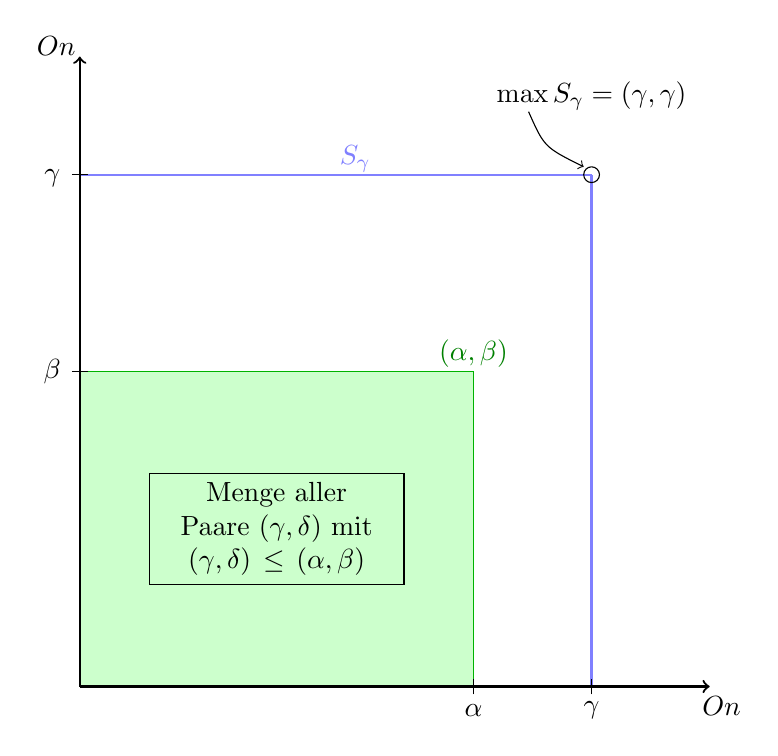
\begin{tikzpicture}
			% S_g + kleiner Zeichen + Kreis + max Schrift
			\draw[thick, blue!50!white] (6.5, 0) -- (6.5, 6.5);
			\draw[thick, blue!50!white] (0, 6.5) -- (6.5, 6.5);
			\draw[blue!50!white] (3.5, 6.7) node {$S_\gamma$};
			
			\draw (6.5, 6.5) circle (0.1);
			\draw (6.5, 7.5) node {$\max S_\gamma = (\gamma,\gamma)$};
			\draw[->] (5.7, 7.3) .. controls (5.9, 6.85) .. (6.4, 6.6);
			
			
			% (alpha, beta) Bereich + Text
			\filldraw[fill=green!20!white, draw=green!70!black] (0, 0) -- (0, 4) -- (5, 4) -- (5, 0) -- (0, 0);
			\draw[green!50!black] (5, 4.23) node {$(\alpha, \beta)$};
			\node[draw, align=center, text width=3cm] at (2.5, 2) {Menge aller Paare $(\gamma,\delta)$ mit $(\gamma,\delta)\leq(\alpha,\beta)$};
			
			% Koordinatensystem
			\draw[->, thick] (0, 0) -- (8, 0); \draw (8.15, -0.25) node {$On$};
			\draw[->, thick] (0, 0) -- (0, 8); \draw (-0.3, 8.13) node {$On$};
			
			
			% gammas auf Koordinatenachsen
			\draw[thin] (6.5, -0.1) -- (6.5, 0.1); \draw (6.5, -0.3) node {$\gamma$};
			\draw[thin] (-0.1, 6.5) -- (0.1, 6.5); \draw (-0.35, 6.45) node {$\gamma$};
			
			% alpha / beta auf Koordinatenachsen
			\draw[thin] (5, -0.1) -- (5, 0.1); \draw (5, -0.3) node {$\alpha$};
			\draw[thin] (-0.1, 4) -- (0.1, 4); \draw (-0.35, 4) node {$\beta$};	
		\end{tikzpicture}
	\end{center}
	\caption{Die grafische Darstellung von $<^\ast$.}
	\label{WohlordnungAufOrdinalHoch2}
\end{figure}

\begin{lemma}
	$<^\ast$ ist eine Wohlordnung.
\end{lemma}
\begin{proof}
	Sei $A\subseteq On\times On$ nicht-leer. Setze $\delta\coloneqq\{\delta'\in On : A\cap S_\delta'\neq\emptyset\}$. Nun ist das Minimum von $A$ das Paar $(\alpha_0,\beta_0)$ mit $\alpha_0\coloneqq\min\{\alpha\in On : \exists\beta[(\alpha,\beta)\in A\cap S_\delta]\}$ und $\beta_0\coloneqq\min\{\beta\in On : (\alpha_0,\beta)\in A\cap S_\delta\}$.
\end{proof}

\begin{definition}
	Die Gödelsche Paarfunktion $G:On\times On\to On$ ist definiert als $G(\alpha,\beta)=otp(\{(\alpha',\beta') : (\alpha',\beta')<^\ast(\alpha,\beta)\}, <^\ast)$. 
	
	Hierbei bezeichnet $otp(A, <)$ die Ordinalzahl $\alpha$ so, dass $(A,<)\cong(\alpha,<)$. Also ist $(\alpha,\beta)\downarrow^{<^\ast}\cong(G(\alpha,\beta), <)$.
\end{definition}

\begin{lemma}
	Es gilt $G(\alpha,\beta)=\{G(\alpha',\beta'):(\alpha',\beta')<^\ast(\alpha,\beta)\}$.
\end{lemma}
Der Beweis zum obigen Lemma lässt sich durch eine Graphik, welche den Isomorphismus von $((\alpha,\beta),<)$ nach $(G(\alpha,\beta), <)$ verdeutlicht.

Damit folgt dann, dass $G$ ordnungserhaltend und injektiv.

\begin{lemma}
	\begin{itemize}
		\item[a)] $G(\alpha, \beta)\geq\max\{\alpha,\beta\}$.
		\item[b)] $G[\alpha\times\alpha]=G(0,\alpha)$. Insbesondere ist $\alpha \leq G[\alpha\times\alpha]$.
		\item[c)] $G[\omega\times\omega]=\omega$.
	\end{itemize}
\end{lemma}
\begin{proof}
	a): $G(\alpha,\beta)=(\{(\alpha',\beta')\in On : (\alpha',\beta')<^\ast(\alpha,\beta)\}, <^\ast)\supset(\{(\gamma,0):\gamma<\alpha\}, <^\ast)\cong(\alpha,<)$. Es folgt, dass $G(\alpha,\beta)\geq\beta$. Analog lässt sich dies für $G(\alpha,\beta)\supseteq\beta$ zeigen.
	
	b): $\alpha\times\alpha=\{(\beta,\gamma)\in On^2 : (\beta,\gamma)<^\ast(0,\alpha)\}$. Nach dem Lemma folgt $G[\alpha\times\alpha]=G(0,\alpha)$ und wegen a) ist $\alpha\leq G(0,\alpha)=G[\alpha\times \alpha]$.
	
	c): Jedes $(m,n)\in\omega\times\omega$ hat nur endlich viele $<^\ast$-Vorgänger, also folgt $G(m,n)<\omega$. Demnach ist $G[\omega\times\omega]\leq\omega$. $G[\omega\times\omega]\geq\omega$ folgt aus b). Also muss $G[\omega\times\omega]=\omega$ gelten. Die Abbildung $G\upharpoonright\omega\times\omega$ ist also eine Bijektion von $\omega\times\omega$ nach $\omega$.
\end{proof}

Nachdem nun einige Hilfsaussagen gezeigt und diskutiert wurden können wir jetzt den Satz von Hessenberg beweisen. Zu Erinnerung: Wir müssen zeigen, dass, basierend auf ZFC, für alle Ordinale $\alpha\geq\omega$ gilt, dass $\alpha\times\alpha\sim\alpha$.
\begin{proof}[Beweis: Satz von Hessenberg]
	Wir wollen dies durch eine transfinite Induktion über $\alpha$ zeigen.
	Induktionsanfang: $\alpha=\omega$: Dies folgt aus dem Teil c) des eben bewiesenen Lemmas.
	
	Für $\alpha>\omega$ lassen sich zwei Fälle aufstellen.
	\begin{itemize}
		\item Falls ein $\beta<\alpha$ existiert mit $\beta\sim\alpha$, dann ist $\alpha\times\alpha\sim\beta\times\beta \stackrel{\text{IV}}{\sim} \beta \sim \alpha$.
		\item Sonst ist $\alpha$ ein Limesordinal, da $\beta+1\sim\beta$ wäre. Mit b) des Lemmas folgt $G[\alpha\times\alpha]\geq\alpha$. Für einen Widerspruch nehmen wir $G[\alpha\times\alpha]>\alpha$ an.
		
		Wähle $(\beta,\gamma)\in\alpha\times\alpha$ mit $G(\beta,\gamma)=\alpha$. Setze $\delta\coloneqq\{\beta,\gamma\}+1$. Also ist $(\beta,\gamma)\in\delta\times\delta$ und $\alpha=G(\beta,\gamma)\in G[\delta\times\delta]$ und daher $\alpha\subseteq G[\delta\times\delta]$.
		
		Nun ist $\alpha\stackrel{(1)}{>}\delta\stackrel{(2)}{>}\omega$, weil (1) $\alpha$ ein Limesordinal ist und (2), weil $\alpha\notin G[\omega\times\omega]$.
		
		Nach der Induktionsvoraussetzung existieren die Bijektion $g:\delta\to\delta\times\delta$ und die Abbildung $h\coloneqq G\circ g : \delta\to G[\delta\times\delta]\supseteq\alpha$.
		
		Die Umkehrabbildung $h^{-1}\upharpoonright\alpha\to\delta$ ist nun aber eine injektive Abbildung von $\alpha$ in eine Teilmenge von $\delta$. Es folgt $\alpha\sim\delta$, also müsste für $\alpha$ eigentlich der erste Fall gelten. Widerspruch!
	\end{itemize}
	
	Es gilt also $G[\alpha\times\alpha]=\alpha$ und damit ist $G\upharpoonright\alpha\times\alpha$ eine Bijektion von $\alpha\times\alpha$ nach $\alpha$.
\end{proof}

Es wurde nun also gezeigt, dass aus dem Wohlordnungssatz, daher auch dem Auswahlaxiom, die eben bewiesene Eigenschaft folgt. Die Umkehrung lässt sich aber auch zeigen.

\begin{satz}[Tarski, 1924]
	In ZF gilt: Die Aussage, dass $a\times a\sim a$ für alle unendlichen Mengen $a$ gilt impliziert das Auswahlaxiom
\end{satz}
\begin{proof}
	Sei $a$ eine Menge und $\beta\in On$ so, dass keine Surjektion von $a$ nach $\beta$ existiert. Nach Voraussetzung gilt $f:a\cup \beta \to (a\cup \beta)\times(a\cup\beta)$. Nun konstruieren wir eine Wohlordnung auf $a$.
	
	Beobachtung: $\beta\times\{x\}\not\subseteq f[a]$, denn sonst ist $h:a\to \beta\times\{x\}\to \beta$ surjektiv. Widerspruch!
	
	Also $S_b\coloneqq\{\gamma\in\beta : f(\gamma)\in\beta\times\{b\}\}\neq\emptyset$.
	
	Damit ist die Funktion $g:a\to\beta, x\mapsto \min S_x$. Dies  ist injektiv und wohldefiniert, denn $S_c\cap S_d=\emptyset$ für $c\neq d\in a$ und $g$ induziert eine Wohlordnung auf $a$ durch:
	$$b<c\text{ gdw. } g(n)<g(c).$$

	Damit wurde eine Wohlordnung gefunden und der Satz von Tarski ist bewiesen.
\end{proof}

Aus dem Satz von Hessenberg lassen sich einige Eigenschaften folgern.

Für $\kappa\in Cn$ und $\kappa\leq\lambda\in Cn^\infty$ gilt $\kappa+\lambda=\kappa\cdot\lambda=\lambda$. 
Dies lässt sich daran sehen, dass $\lambda \leq \kappa+\lambda\leq\lambda+\lambda \leq 2\cdot\lambda =\lambda$ bzw. $\lambda \leq \kappa\cdot\lambda \leq \lambda\cdot\lambda = \lambda$.

Weiter gilt für $n\geq 1$ und $\lambda \in Cn^\infty$, dass $\lambda^n=\lambda$.

\begin{satz}
	\begin{itemize}
		\item[a)] $\vert \Pot{x} \vert = 2^{\vert x \vert}$.
		\item[b)] Wenn $2\leq \kappa \leq \lambda$ mit $\kappa\in Cn, \lambda\in Cn^\infty$, dann ist $\kappa^\lambda=2^\lambda$.
	\end{itemize}
\end{satz}
\begin{proof}
		a): $\Pot{x}\sim\{f:x\to2\}$ und nach Definition ist $\vert\{f:x\to 2\}\vert=2^{\vert x \vert}$.
		
		b): $2^\lambda \leq \kappa^\lambda \leq 2^{\lambda\cdot\lambda}=2^\lambda$.
\end{proof}

Durch weitere Überlegungen kann man feststellen, dass $\vert \mathbb{Q} \vert=\vert \omega\times\omega \vert = \omega$ und $\vert \mathbb{R} \vert = \omega^\omega = 2^\omega=\vert \Pot{\mathbb{N}}\vert$. Und mit Hilfe von Satz \ref{SatzVonCantor} folgt, dass $\vert \mathbb{R} \vert \neq \vert \mathbb{Q} \vert$.

\subsubsection{Die Kontinuumshypothese (CH)}

Die Kontinuumshypothese (englisch: continuum hypothesis) besagt, dass $\omega^+=2^\omega$ oder anders ausgedrückt: $\aleph_1=2^{\aleph_0}$. Zusätzlich gibt es auch die verallgemeinerte Kontinuumshypothese (GCH), nach welche $\aleph_\alpha+1=2^{\aleph_\alpha}$ für alle $\alpha\in On$ gilt.
\par

Es lässt sich aber zeigen, dass \textit{CH unabhängig von ZFC ist}. Das heißt, es gilt sowohl $ZFC \not\models CH$, als auch $ZFC \not\models \neg CH$, wobei davon ausgegangen wird, dass ZFC konsistent ist und es somit überhaupt ein Modell von ZFC gibt.

Der Beweis dafür wurde von zwei Mathematikern geführt. Der erste Teil wurde von Kurt Gödel im Jahre 1938 bewiesen. Dafür hat er aus dem bekannten Stufenmodell $(S_\alpha)_{\alpha\in On}$ eine konstruierbare Hierarchie $(L_\alpha)_{\alpha\in On}$ erzeugt. Für diese gilt $L_0\coloneqq\emptyset$, für Limesordinale $\lambda$ ist $L_\lambda\coloneqq \bigcup_{\beta<\lambda}L_\beta$ und für $\alpha+1$ ist $L_{\alpha+1}\coloneqq\{x\subseteq L_\alpha : \exists a_1,\dots,a_n\exists\varphi(z,y_1,\dots,y_n) : x=\{z\in L_\alpha : (L_\alpha,\in) \models \varphi(z,a_1,\dots, a_n)\}\}$ die Menge aller Teilmengen, die sich mithilfe einer FO-Formel darstellen lassen.

Damit konnte Gödel folgern, dass $(L,\in)\models ZF$, $(L,\in)\models AC$ und $(L,\in)\models GCH$.
\\
Den zweiten Teil konnte Paul Cohen im Jahre 1963 beweisen. Sein Endresultat war, dass $ZF\notin AC$ und $ZFC \notin CH$.
\\

Daraus folgt also, dass mithilfe von ZFC nichts über die Korrektheit der Kontinuumshypothese aussagen lässt. ZFC ist also nicht vollständig. Zusätzlich nehmen die obigen Überlegungen die Konsistenz von ZFC an.

Trotz dieser Probleme mit ZFC wird dieses als \glqq Standard \grqq{} Axiomensystem angenommen. Wie im nächsten Kapitel nämlich gezeigt werden wird gilt für alle Axiomensysteme, welche genügend Aussagekraft haben, dass deren Konsistenz nicht gezeigt werden kann und sie nicht vollständig sein können.
